% Compile with XeLaTeX (twice), or tectonic main.tex.
\documentclass[11pt,a4paper]{article}
\usepackage[margin=25mm]{geometry}
\usepackage{fontspec}
\setmainfont{lmroman10-regular.otf}[BoldFont=lmroman10-bold.otf,
 ItalicFont=lmroman10-italic.otf,BoldItalicFont=lmroman10-bolditalic.otf]
\setsansfont{lmsans10-regular.otf}[BoldFont=lmsans10-bold.otf,
 ItalicFont=lmsans10-oblique.otf]
\setmonofont{lmmono10-regular.otf}[Scale=MatchLowercase]
\usepackage{amsmath,amssymb}
\usepackage{graphicx,booktabs,longtable,array,calc}
\usepackage{caption,subcaption,float,placeins}
\usepackage{etoolbox,titlesec,microtype,ragged2e}
\usepackage{xcolor}
\usepackage[unicode,hidelinks]{hyperref}
\usepackage{bookmark,newunicodechar}
\newunicodechar{→}{\ensuremath{\rightarrow}}
\newunicodechar{≤}{\ensuremath{\leq}}
\newunicodechar{≥}{\ensuremath{\geq}}
\newunicodechar{≠}{\ensuremath{\neq}}
\newunicodechar{−}{\ensuremath{-}}
\newunicodechar{μ}{\ensuremath{\mu}}
\newunicodechar{±}{\ensuremath{\pm}}
\providecommand{\tightlist}{\setlength{\itemsep}{0pt}\setlength{\parskip}{0pt}}
\providecommand{\pandocbounded}[1]{#1}
\setcounter{secnumdepth}{4}
\setcounter{tocdepth}{3}
\titleformat{\section}{\large\bfseries}{\thesection}{0.7em}{}
\titleformat{\subsection}{\normalsize\bfseries}{\thesubsection}{0.7em}{}
\titleformat{\subsubsection}{\normalsize\bfseries}{\thesubsubsection}{0.7em}{}
\titleformat{\paragraph}[block]{\normalsize\itshape}{\theparagraph}{0.7em}{}
\titlespacing*{\paragraph}{0pt}{1.2ex plus .3ex}{.5ex}
% User-selected block paragraphs: flush left, with a blank line between paragraphs.
\setlength{\parindent}{0pt}
\setlength{\parskip}{\baselineskip}
\setlength{\emergencystretch}{2em}
\captionsetup{font=small,labelfont=bf,skip=6pt}
\captionsetup[table]{position=top}
\AtBeginEnvironment{longtable}{\small\renewcommand{\arraystretch}{1.15}}
\setlength{\tabcolsep}{4pt}
\setlength{\LTpre}{8pt}
\setlength{\LTpost}{8pt}
\renewcommand{\topfraction}{.95}
\renewcommand{\bottomfraction}{.8}
\renewcommand{\textfraction}{.05}
\renewcommand{\floatpagefraction}{.8}
\widowpenalty=10000
\clubpenalty=10000
\hypersetup{pdftitle={Consistency Models in Distributed Databases},
 pdfauthor={Chen Luwei, Dai Peisong, Wan Sihan}}
\begin{document}
\hypersetup{pageanchor=false}
\begin{titlepage}
\centering
\vspace*{25mm}
{\large National University of Singapore\par}
\vspace{15mm}
{\large DSA5208\par}
\vspace{3mm}
{\large Scalable Distributed Computing for Data Science\par}
\vspace{3mm}
{\large Project I\par}
\vspace{20mm}
{\Large\bfseries\mbox{Consistency Models in Distributed Databases}\par}
\vspace{20mm}
{\small\mbox{Chen Luwei (A0352040X)\quad Dai Peisong (A0351174J)\quad Wan Sihan (A0356906U)}\par}
\vfill
{\large 26 September, 2026\par}
\vspace*{15mm}
\end{titlepage}
\pagenumbering{roman}
\hypersetup{pageanchor=true,linktoc=all}
\pdfbookmark[0]{Contents}{contents}
\begingroup
\setlength{\parskip}{0pt}
\tableofcontents
\endgroup
\clearpage
\pagenumbering{arabic}
\section{Introduction}\label{introduction:introduction}

In this project, we aim to explore how Cassandra, a distributed database, handles different types of client-centric consistency observed by applications. The consistency models to be tested are read-your-writes (RYW), monotonic-reads (MR), monotonic-writes (MW), and writes-follow-reads (WFR)~\cite{terry1994}. We first set up a replicated distributed database with three Docker containers forming a Cassandra cluster, then explored its consistency behaviours by tuning the read consistency level, the write consistency level~\cite{cassandra-dynamo}, and artificially injected replication latency. For each consistency model, we first derive a prediction based on the condition R + W \textgreater{} N, then construct a test in which a single client writes and reads through different coordinator nodes, and finally measure the fraction of trials that violate the guaranteed consistency.

Note that the tests are repeated under several settings, including normal, one node failure, and a network partition that blocks an individual node, to represent different levels of network availability. Our results show that delayed propagation exposed read-your-writes and monotonic-reads violations under weak consistency settings, while stronger settings prevented these observed anomalies in successful trials but reduced availability during failures and partitions. In the monotonic-writes and writes-follow-reads tests, deliberately inverted timestamps caused earlier values to prevail over later updates, even at stronger consistency levels. These findings highlight the distinct roles of replica visibility, availability, and timestamp ordering within the tested workloads, rather than establishing general consistency guarantees.

\subsection{System Configuration}\label{introduction:system-configuration}

{
\begin{table}[H]
\centering
\small
\renewcommand{\arraystretch}{1.15}
\caption{System configuration and software environment.}\label{tab:introduction-1}
\begin{tabular}{@{}
  >{\RaggedRight\arraybackslash}p{(\linewidth - 2\tabcolsep) * \real{0.2300}}
  >{\RaggedRight\arraybackslash}p{(\linewidth - 2\tabcolsep) * \real{0.7700}}@{}}
\toprule\noalign{}
\begin{minipage}[b]{\linewidth}\RaggedRight
Component
\end{minipage} & \begin{minipage}[b]{\linewidth}\RaggedRight
Configuration
\end{minipage} \\
\midrule\noalign{}
Host & Lenovo Thinkbook 16p, Linux {[}6.18.33.2-microsoft-standard-WSL2 x86\_64{]}, Docker {[}29.7.2{]}; Macbook Pro, Darwin 27.0.0 arm64, Docker {[}28.4.0{]} \\
Database & Apache Cassandra {[}4.1.12{]} \\
Client & Windows/WSL2: Python {[}3.11.16{]}, macOS: Python {[}3.12.2{]}; Cassandra-driver {[}3.30.1{]} both \\
Keyspace & consistency\_lab, replication factor=3, SimpleStrategy \\
Table & kv(key text PRIMARY KEY, value int, writer text) with read\_repair=NONE, speculative\_retry=NONE~\cite{cassandra-read-repair,cassandra-ddl} \\
Consistency Levels & ONE, QUORUM, ALL (requiring responses from 1, 2, and 3 replicas, respectively; $N=3$). \\
\bottomrule
\end{tabular}
\end{table}
}

Here, we disabled two default settings, read repair and speculative retry, because both would mask the divergence we want to observe. Read repair writes the newest value back to stale replicas as part of a read request, so a violation seen once would be repaired before we could observe it again. Speculative retry will try to contact extra replicas when one responds slowly, which the injected latency would trigger constantly, making CL=ONE behave just like a larger CL.

In particular, to make the role of each node in the cluster clear, each client session is pinned to a chosen node through a white-list mechanism~\cite{driver-policies}. This allows us to identify and keep track of the coordinator for every read/write request.

\subsection{Cluster and Network Setup}\label{introduction:cluster-and-network-setup}

The cluster consists of three containers (cass1, cass2, and cass3) on one Docker bridge network, with cass1 serving as the seed node. Each node's CQL port 9042 is published on the host as port 9042, 9043, and 9044, respectively. The nodes communicate with one another through port 7000 inside the bridge network.

We initialize the experiment with \verb|scripts/bootstrap.sh|. It starts the cluster using Docker Compose, waits for the containers to become healthy, and checks their status with \verb|nodetool|. It then runs \verb|scripts/setup_keyspace.cql| on cass1 to create the \verb|consistency_lab| keyspace and the \verb|kv| table, retrying if Cassandra is not yet ready. The script creates a Python virtual environment in \verb|.venv|, installs the packages in \verb|requirements.txt|, tests the client connections, and records the software and host information in \verb|results/environment.txt|.

After bootstrap, we use \verb|scripts/inject_latency.sh| to apply Linux \verb|tc/netem| delay to outgoing traffic destined for port 7000 on each container. The default setting is 200 ms of delay with 50 ms of jitter. This affects internode communication, including replication and internode read traffic, while leaving the client-facing CQL ports untouched. Delaying client traffic could add time between a completed write and the subsequent read, allowing more time for propagation and changing the measured violation rate.

A node failure scenario is realized by simply stopping cass3. Meanwhile, a network partition is realized by dropping traffic on port 7000 between cass3 and the other two nodes in both directions, leaving cass3 running with its client port accessible; clients can therefore access both the majority side (cass1, cass2) and the minority side (cass3).

Finally, as we aim to emulate replication delay and node partitions rather than independent machine failures, we run all three containers on a single physical host, sharing the same system clock, within Docker Desktop's Linux environment, while the client runs directly on the host operating system.

\begin{figure}[H]
\centering
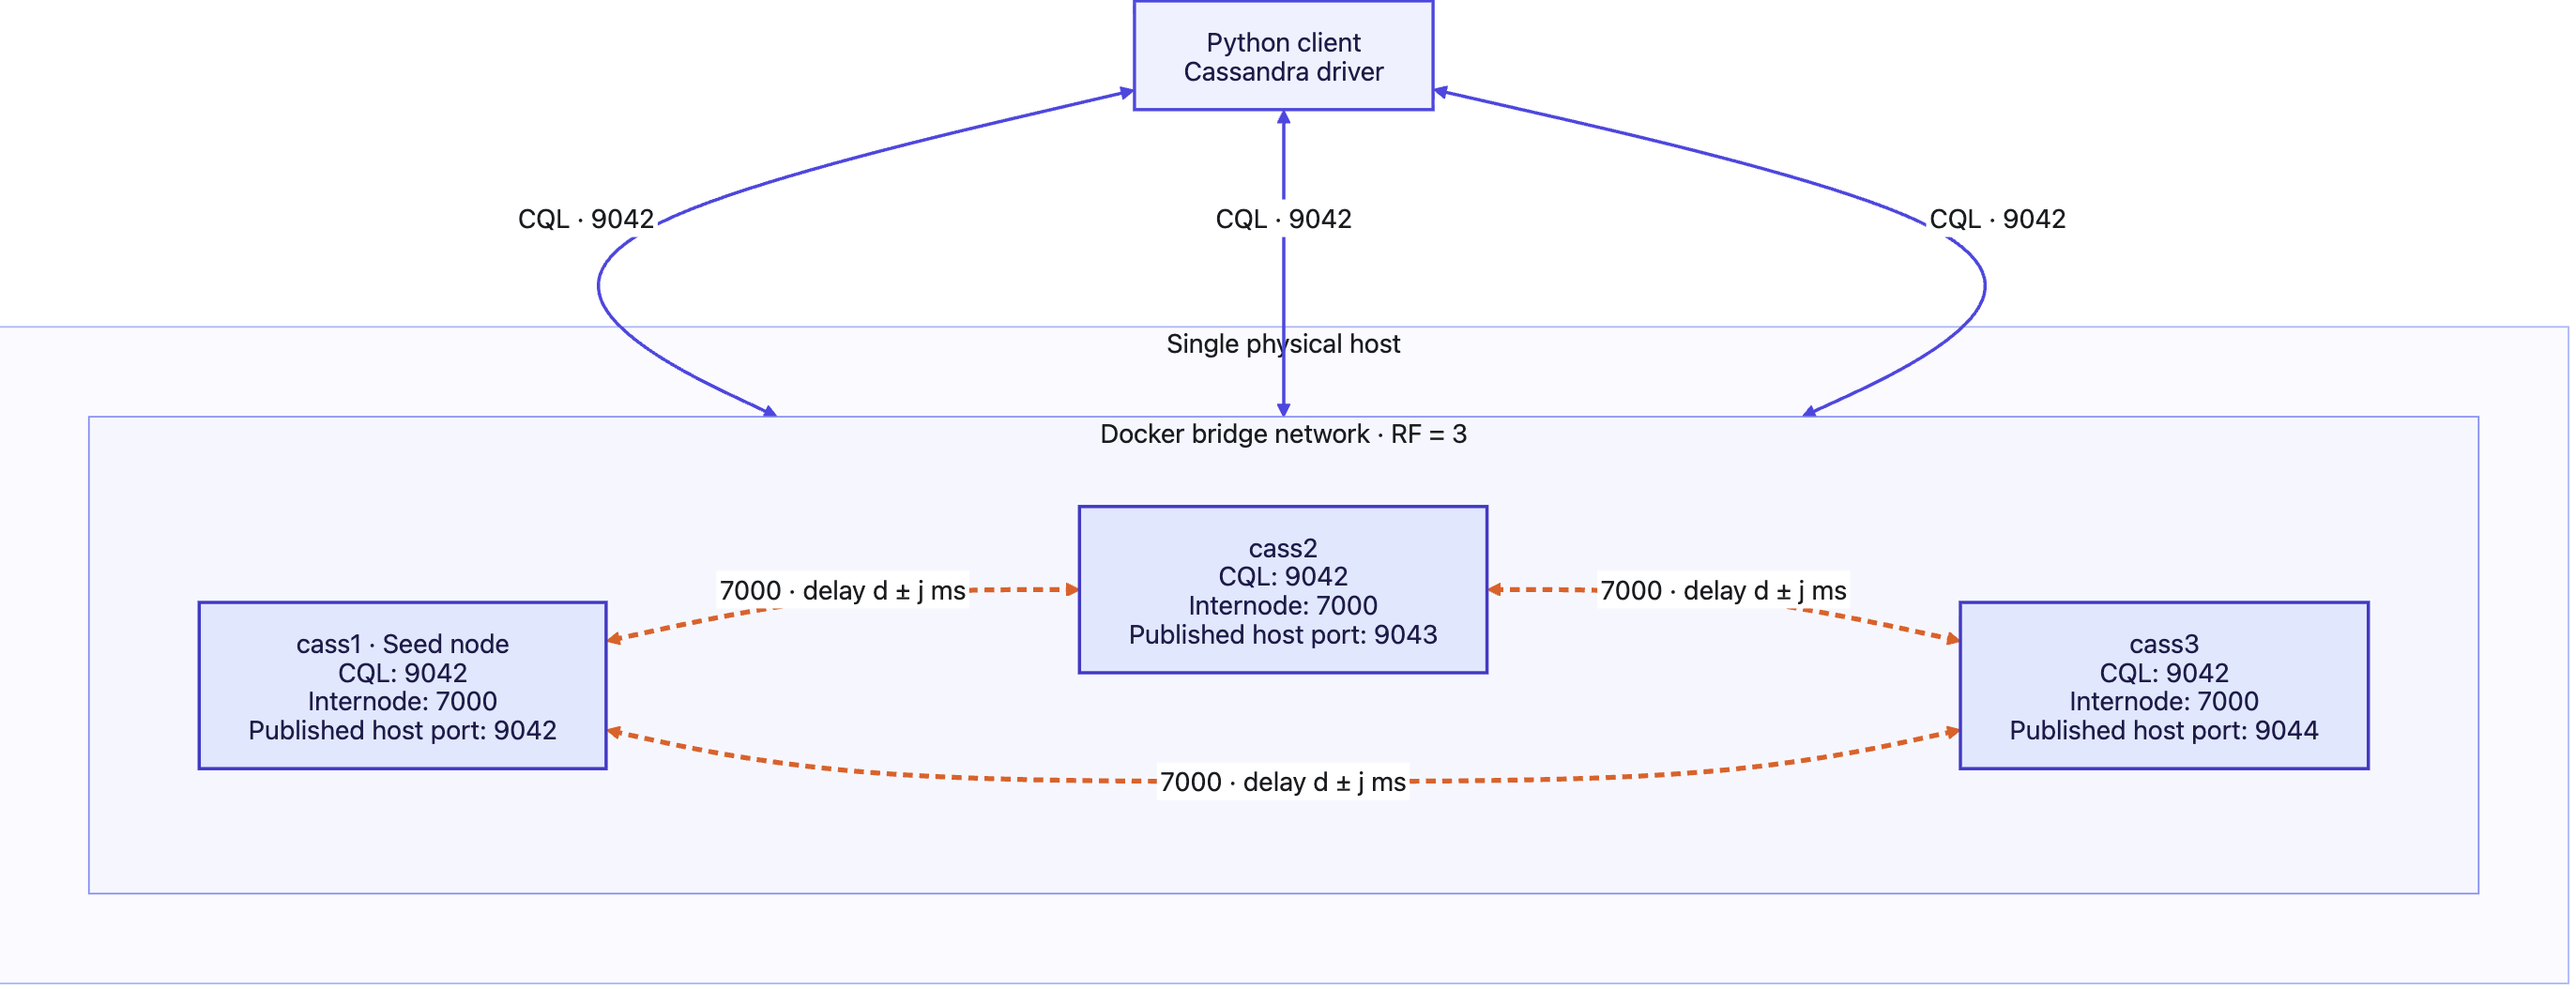
\includegraphics[width=\linewidth]{figures/architecture.png}
\caption{Three-node Cassandra cluster and communication ports.}
\label{fig:architecture}
\end{figure}

\section{Consistency Test}\label{introduction:consistency-test}

\subsection{Read-your-Writes Consistency}\label{ryw:read-your-writes-consistency}

\subsubsection{Definition}\label{ryw:definition}

Read-your-writes (RYW) consistency guarantees that once a client's write has completed, all subsequent reads by that client observe that write or a later version. Namely, suppose a client writes \emph{x=i} and the write completes successfully. If the same client subsequently reads \emph{x} and obtains \emph{i}, then read-your-writes consistency is preserved. In contrast, if the read returns no value because it reaches a replica that has not yet received the write, the client cannot observe its own completed write, constituting an RYW violation.

\subsubsection{Experimental Design}\label{ryw:experimental-design}

This section aims to investigate how Cassandra handles read-your-writes consistency under different combinations of write and read consistency levels denoted as \emph{W} and \emph{R}, respectively. For each iteration, the script generates a new key and performs one write followed immediately by one read from the same client. The write and read are deliberately sent through different coordinator nodes: by default, the client writes through cass1 and subsequently reads the same key through cass2. This avoids trivially reading the newly written value from the same coordinator and represents situations in which a client reconnects to another node, is redirected by a balancer, or experience driver failover.

For iteration \emph{i}, the client first writes \emph{value=i} to a fresh key using the specified write consistency level \emph{W,} including ONE, QUORUM, and ALL. Once the write has completed successfully, the client immediately reads the same key through the designated read coordinator using consistency level \emph{R}. It is worth noting the architecture of our cluster indicates no artificial waiting period introduced between the two operations but communication between nodes. Then, the outcome of each iteration is classified as a preservation of RYW when \emph{R(x)=i} or a violation against RYW when \emph{R(x)≠i}.

In particular, we use a fresh key in every iteration, making the violation criterion unambiguous. When the write has been confirmed but has not yet become visible to the replicas serving the subsequent read, the read returns None, which will be recorded as a violation. Meanwhile, such implementation also enables us to record a less common case in which a non-null value different from \emph{i} is observed.

\begin{figure}[H]
\centering
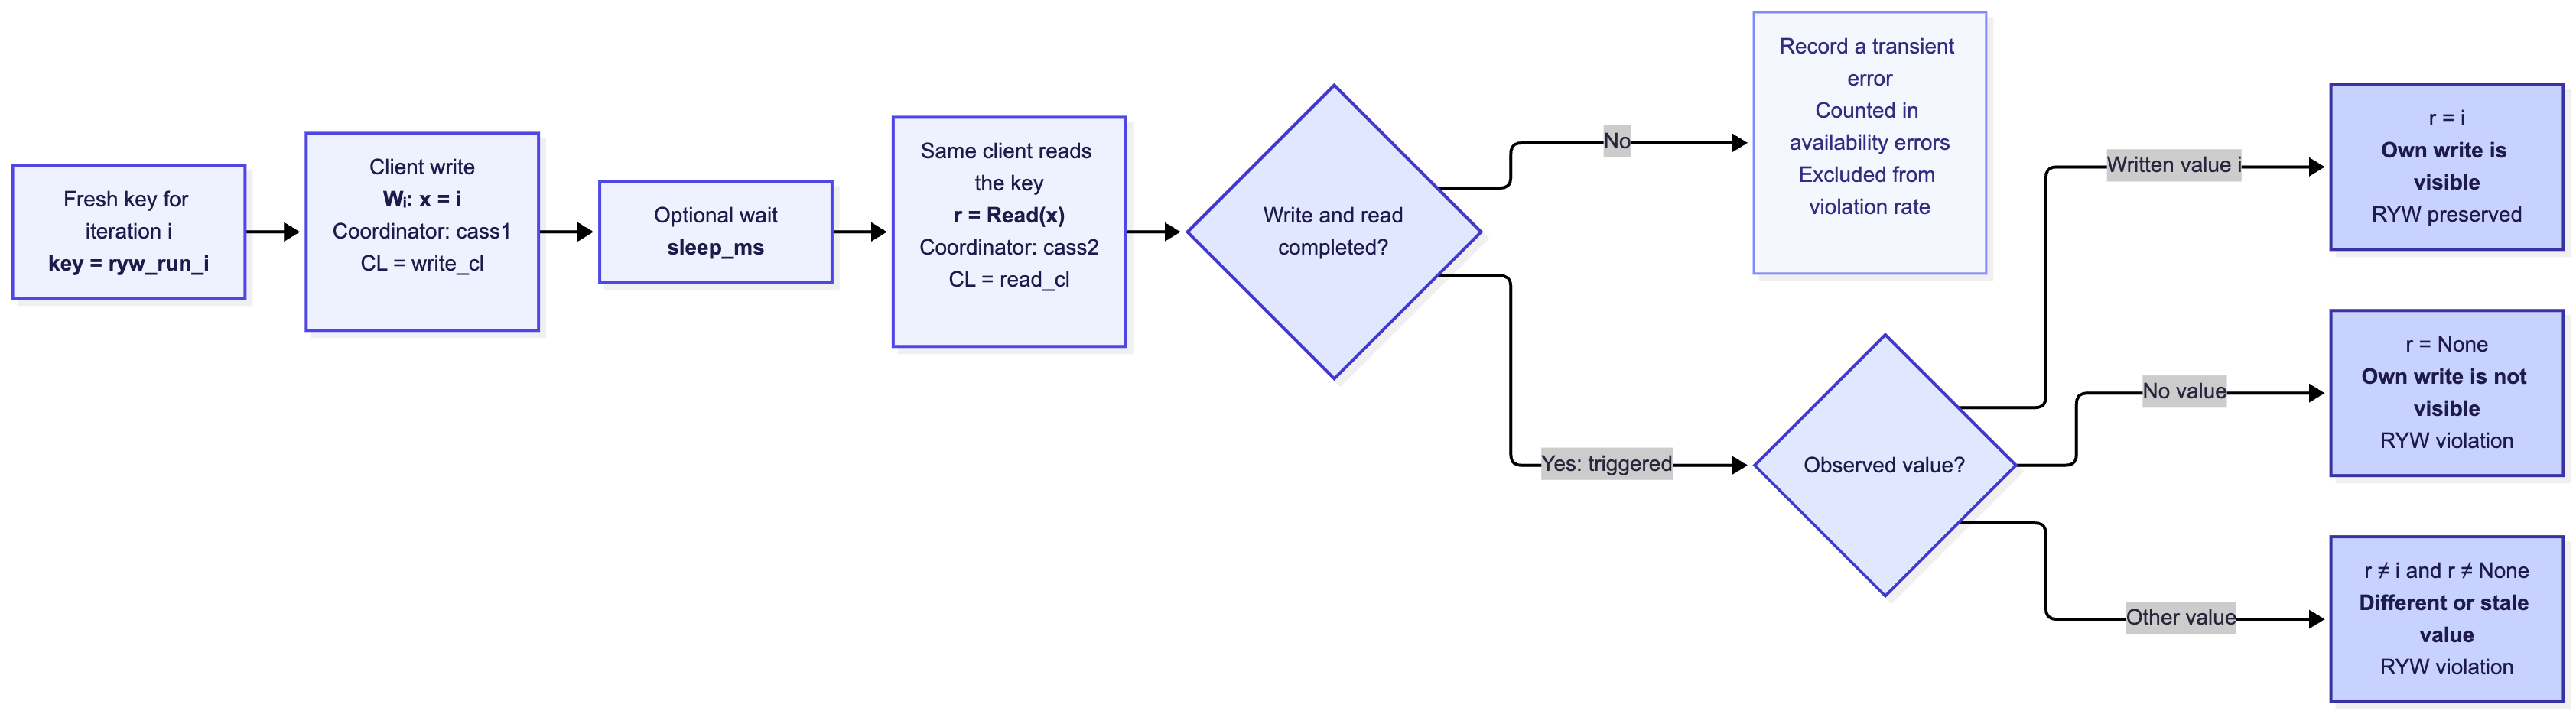
\includegraphics[width=\linewidth]{figures/ryw_flow.png}
\caption{Read-your-writes experimental workflow.}
\label{fig:ryw-flow}
\end{figure}

We will detail the combinations of Cassandra consistency levels in the following:

{
\begin{table}[H]
\centering
\small
\renewcommand{\arraystretch}{1.15}
\caption{RYW consistency-level combinations and replica-set intersection conditions (RF=3).}\label{tab:ryw-1}
\begin{tabular}{@{}lll@{}}
\toprule\noalign{}
Write CL & Read CL & Quorum Relationship (RF=3) \\
\midrule\noalign{}
ONE & ONE & 1+1≤3 \\
ONE & QUORUM & 1+2=3 \\
QUORUM & QUORUM & 2+2\textgreater3 \\
ALL & ONE & 3+1\textgreater3 \\
\bottomrule
\end{tabular}
\end{table}
}

For each configuration above, the test is repeated for the specified number of iterations, and the RYW violation rate is calculated over successfully completed write-read trials. Cassandra timeout or availability exceptions are recorded separately as errors rather than being counted as consistency violations. Each trial additionally records the write and read coordinators, the generated key, written and observed values, and the write timestamp, allowing individual violations to be inspected afterwards.

One last significant component is the injected latency, as we hope to examine how the RYW violation rate changes as the replication window increases. Particularly, we expect weaker consistency-level combinations, like (ONE, ONE) to be more susceptible to violations than the stronger ones.

\subsubsection{Principle and Key Implementation}\label{ryw:principle-and-key-implementation}

The implementation tests visibility after an acknowledged write, rather than the order of competing overwrites. For each fresh key $k_i$, the client waits for the write of value $i$ to complete before issuing the read. In the delay sweep, no additional client-side sleep is inserted. The predicate is $r_i\ne i$, where $r_i$ is the returned value and an absent row is represented by \texttt{None}. Because there is no intentional competing write to the key, equality with $i$ is sufficient for the successful outcome in this workload.

Coordinator selection is controlled through the node-pinned sessions described in Section~\ref{introduction:system-configuration}. Changing the coordinator does not force a particular replica to answer: the read coordinator still selects replicas according to Cassandra's read path. The injected delay targets internode traffic on port 7000, not client CQL traffic on port 9042. This separates the manipulated internode delay from an artificial wait between the client's write and read, although internode read exchanges are also affected.

Let $N=3$ be the replication factor, and let $W$ and $R$ denote the required numbers of write acknowledgements and read responses. For a successful write followed by a successful read of this fresh key, $W+R>N$ forces the read response set to intersect the write acknowledgement set. This supports the expected visibility of the written value for QUORUM/QUORUM and ALL/ONE in this workload. When $W+R\leq N$, intersection is not guaranteed; this permits stale reads but does not determine their frequency. It is not a general proof of all client-centric consistency properties.

Only trials in which both operations complete enter the RYW violation-rate denominator. Timeout and availability exceptions are logged separately, so a failed operation is not classified as either a preserved or a violated read. The reported percentage is
\begin{equation}
\text{RYW violation rate (\%)} =
100\,\frac{\#\{\text{completed trials with }r_i\ne i\}}
{\#\{\text{completed write--read trials}\}}.
\end{equation}
If no trial completes, the rate is undefined rather than zero. The per-iteration trace records the written and observed values, coordinator identities, and any operation error, supporting inspection of individual outcomes.

\subsubsection{Predicted Outcomes}\label{ryw:predicted-outcomes}

Now, we may infer potential outcomes based on the Cassandra read/write consistency levels with corresponding quorum relationship, replication factor, and injected latency. For (ONE, ONE) configuration, we expect it to generate the highest violation rate. In our setup, writes are coordinated by cass1 by default, whereas subsequent reads are coordinated by cass2. Then, such design enables the subsequent read to be served before the newly written value has been copied to the replica. Meanwhile, increasing inter-replica latency may enlarge the window in which an RYW violation can be observed.

For (ONE, QUORUM), we expect violations to remain nontrivial because the exact quorum relationship implied here, 1+2=3=RF, creates a boundary case in which the write and the read replica sets are not guaranteed to overlap. However, requiring a quorum of two replicas for each read increases the likelihood that at least one responding replica has received the latest write, including the write coordinator that holds a local replica. We therefore expect a lower violation rate than under (ONE, ONE), although the rate may still increase with replication latency as the window widens.

For (QUORUM, QUORUM), given that the quorum relationship implies an overlap between the write and read replica sets, a subsequent read following a successful write must include at least one replica that has received the latest write. Cassandra can then reconcile the returned versions based on their timestamps and select the latest value. Therefore, we expect RYW violation to be absent, regardless of the latency level. Similar reasoning may apply to (ALL, ONE). With RF=3, a write consistency level of ALL would request all three replicas to acknowledge the write, then any subsequent read must observe the latest written value. The latency level here will be irrelevant to the consistency outcome but completion time.

\subsubsection{Results and Analysis}\label{ryw:results-and-analysis}

\begin{figure}[H]
\centering
\begin{subfigure}{\linewidth}
\centering
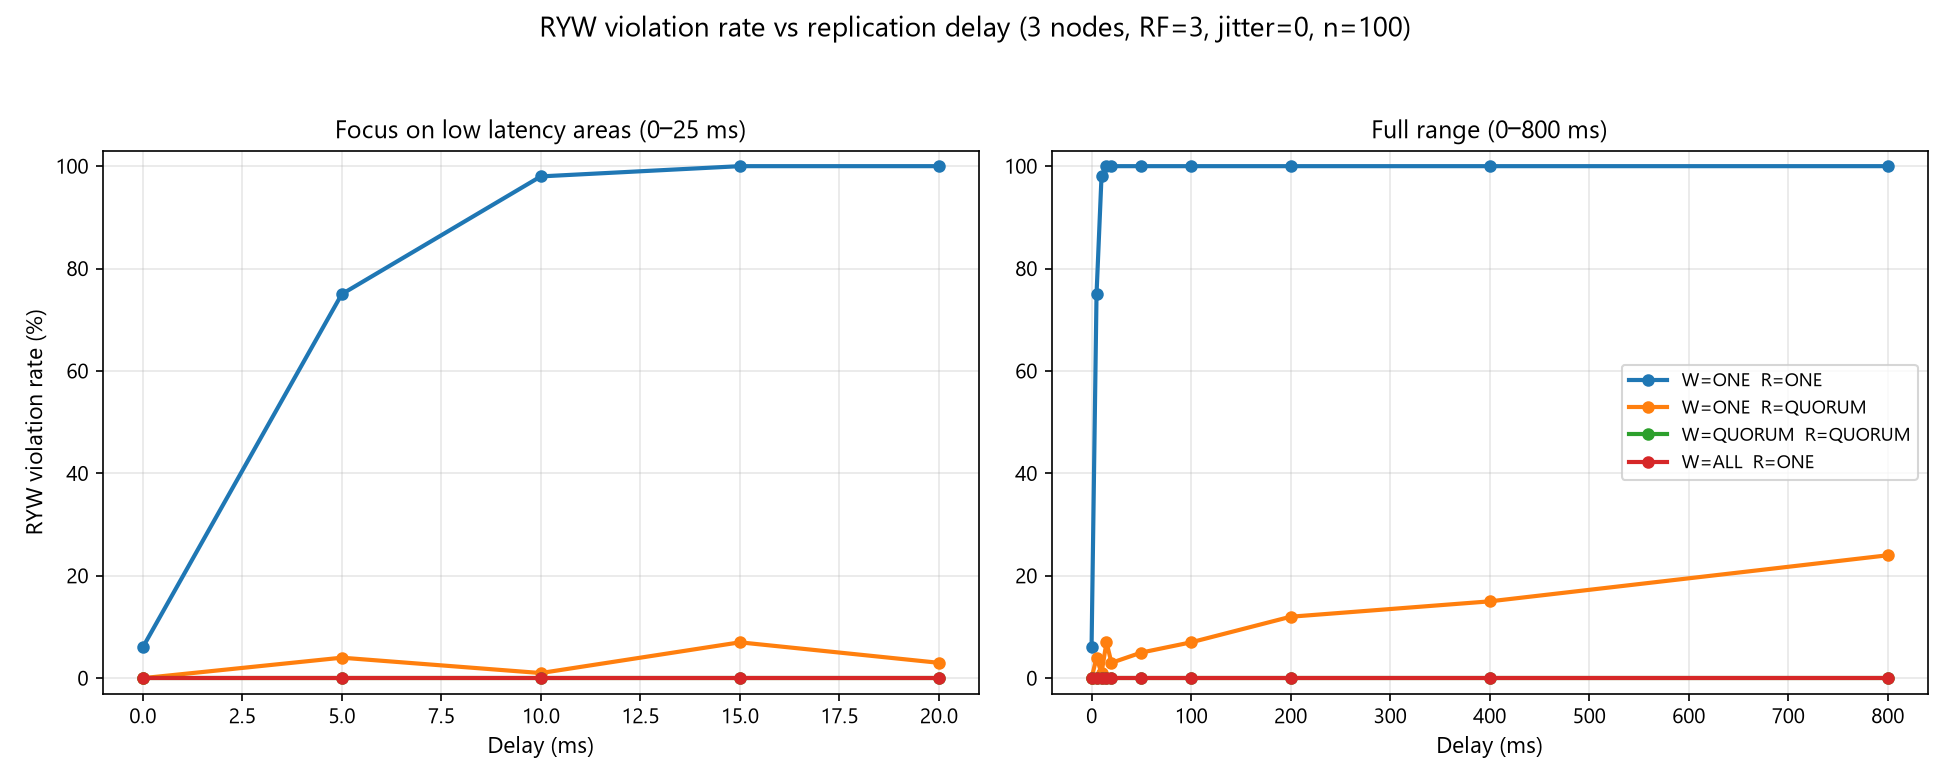
\includegraphics[width=\linewidth]{figures/ryw_macos.png}
\caption{macOS}
\end{subfigure}
\par\medskip
\begin{subfigure}{\linewidth}
\centering
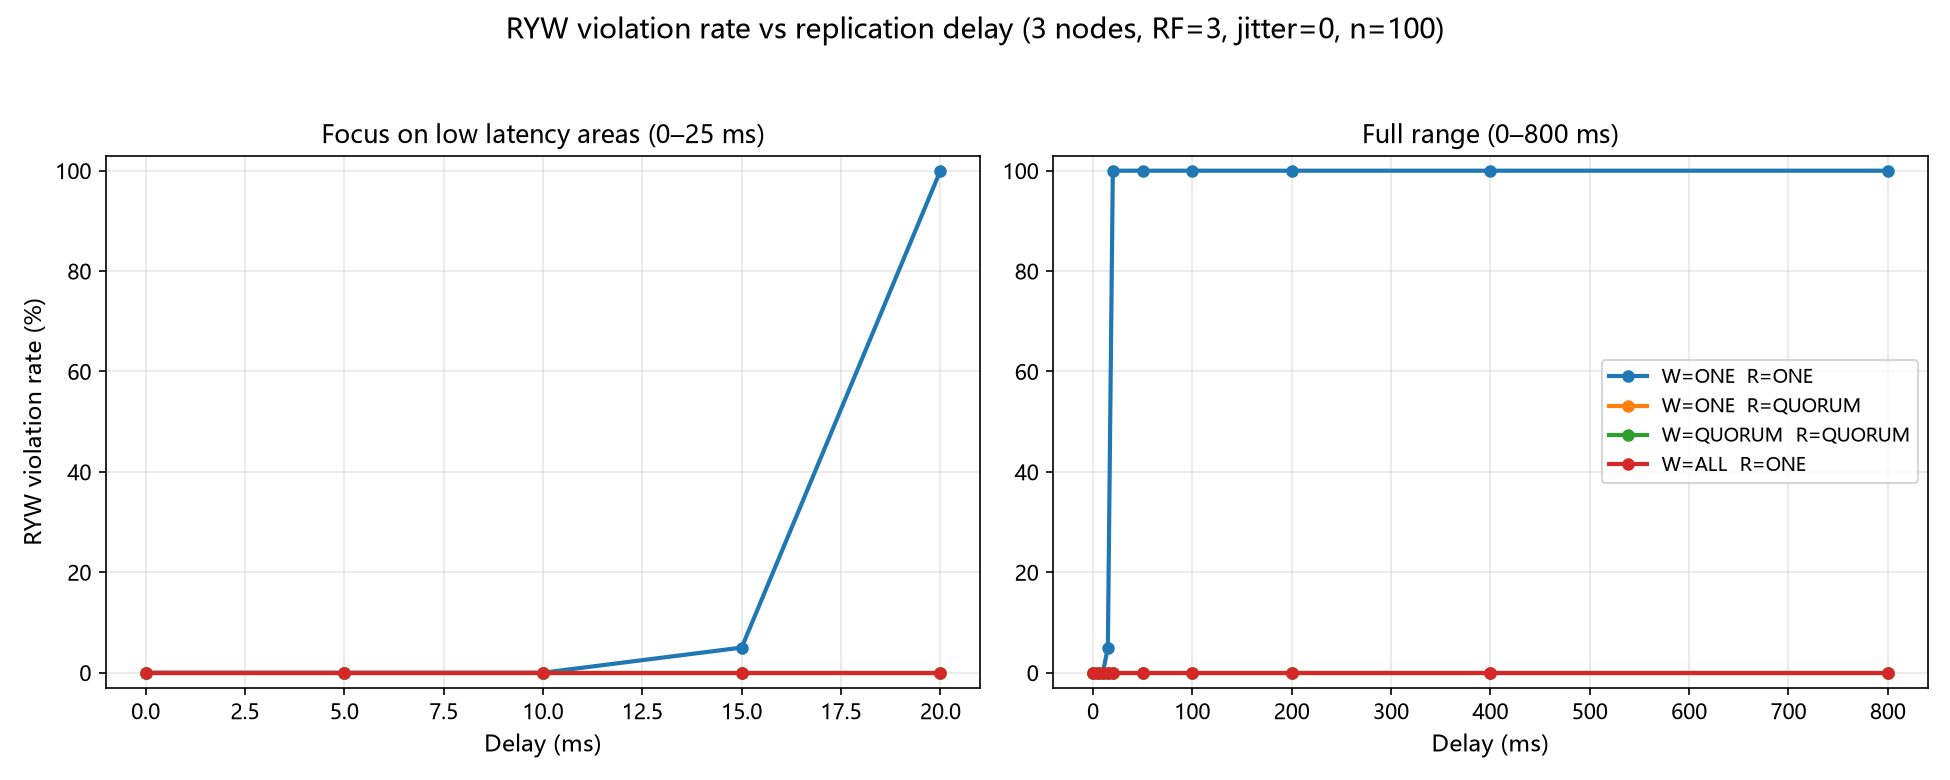
\includegraphics[width=\linewidth]{figures/ryw_windows.png}
\caption{Windows}
\end{subfigure}
\par\medskip
\caption{Comparisons between read-your-writes (RYW) consistency behaviours by hosts on macOS and Windows}
\label{fig:ryw-comparison}
\end{figure}

In order to test RYW consistency in a more heterogeneous environment, we ran the same test on both Windows and macOS hosts, hoping to see whether differences in the underlying operating system and Docker execution would introduce observable variance beyond the general behaviours expected from Cassandra itself. Indeed, while two settings gave similar overall patterns across consistency levels, we did find nuances in their measured violation rates and transition points as latency grows. Nevertheless, we will first interpret the general behaviours shown in the following figure before discussing these platform-specific findings.

As suggested by Figure {[}3{]}, the effect of replication latency on RYW consistency depends strongly on the chosen write and read consistency levels. The most observable effect occurs under (ONE,ONE) setting. Without injected delay, the violation rate remains relatively low, and we attribute such effect to the fact that intra-replica communication moves faster than the time lapse between two consecutive write and read requests from the client's end. However, once a small delay is introduced, it rises sharply and further converges to 100\% no later than 20ms. Disregarding jitters and hardware variance, we may interpret this decisive latency level threshold as a rough approximation of the time difference between the point where the replication is finished and accessible to the coordinator and the point when the read request arrives. Beyond this level, we found any further increases in latency produce nearly no additional change, indicating that the violation rate has effectively saturated. This behaviour is actually consistent with the weak overlapping relationship between write and read replica sets of (ONE, ONE), as introducing larger latency will enlarge the window in which a subsequent read may be satisfied before the latest write has propagated successfully.

Another material pattern is observed under (ONE, QUORUM). As expected, violations remain well below those of (ONE, ONE) and still preserve a nearly non-decreasing relationship with latency level. However, at higher latency, the violation rate rises steadily rather than converging sharply. This is also consistent with the boundary quorum relationship, where W+R=1+2=3=RF, under which overlap between the write and read replica sets is possible but not surely guaranteed. Requiring two replica responses nevertheless has a non-trivial probability that the read request is handled by a replica containing the last write. It is further suggesting that the fluctuations in high latency regime can be explained by not only the replica participation of individual requests but the timing, where the latter factor was indeed dominated by the former one.

In contrast, (QUORUM, QUORUM) and (ALL, ONE) gave us no substantial violations throughout the tested latency range. This is again consistent with our inference on quorum relationship and it indicates that the injected latency for replication is now independent of the write/read consistency level but solely of how fast these operations will be completed.

Finally, we can proceed to discuss the cross-platform differences separately as variations in the execution and request-handling schemes rather than as changes to these underlying consistency relationships. We repeated the delay sweep tests on a Windows host and a macOS host (n=100, jitter=0). The two platforms agree on the general pattern, where combinations (QUORUM, QUORUM) and (ALL, ONE) stay at 0\% at every delay, and (ONE, ONE) converges to 100\% in high-latency regime. However, two platforms differ in where the other two configurations rise. On one hand, for (ONE, ONE), macOS is already at 75\% at 5ms whereas Windows shows no violation up to 10ms. On the other, Windows shows no violation at all for (ONE, QUORUM), while macOS shows nearly 8\% at delays of 5ms and above. Yet the absence of violations under (ONE, QUORUM) on Windows is not general because when we later introduced jittered delay, we observed the same host violates in 1.5\% (10ms delay, 10ms jitter), 14.5\% (50ms delay, 50ms jitter) and 19.3\% (100ms, 50ms), a seemingly compound effects from delay-jitter combinations.

To figure out where these cross-platform differences come from, we composed a diagnostic version of the RYW test (experiments/ryw\_diagnostic.py) that runs the same sequence but enables Cassandra query tracing for both requests and stores one JSON record per iteration, including the platform, read/write coordinator, replica addresses, client-end timestamp, etc. By detailing these factors, we are able to answer questions like which replica the read coordinator asked for and when each message left one node and reached the next. Interestingly, it is in these answers that we figured out potential explanations of those differences.

We ran the diagnostic script for (ONE, QUORUM) on both hosts (100ms, n=20). Both runs showed a 1/20 violation rate, and while these numbers are too few to be statistically significant, tracing how they work shows the mechanism. Normally, the read coordinator, cass2, reads its own copy, then asks one other replica for a digest. Asking cass1 always finds the row, yet asking cass3 is a race between the replication and the digest request, and a violation only happens when the digest request wins.

The replication leaves cass1 as soon as the write is processed, while the digest request only leaves cass2 after the client's write is acknowledged. Because that write call took much longer on Windows (13.8ms median vs.~4ms on macOS), the digest request also starts later on Windows, giving the replication roughly 10ms more time to arrive first. This is also consistent with the observation we had on (ONE, ONE), where the violation rate only starts to rise when the injected latency is larger than 10ms.

Additionally, we may bring up another minor yet inspiring finding that the two hosts don't pick the same replica as often. Out of our 20 reads in our diagnostic test, cass2 asked cass1 for a digest 15 times on Windows but only 7 times on macOS, nudging Windows toward fewer violations. This choice is made by Cassandra's dynamic snitch based on observed replica latency, rather than directly by the client. However, with only 20 samples per run, we cannot rule out sampling noise as an explanation for the observed split.

\subsubsection{Limitations}\label{ryw:limitations}

These results are specific to our three-container setup and the tested request paths. Pinning a coordinator does not fix which replicas answer a read, and the delay applied to port 7000 affects internode read traffic as well as write propagation. We disabled read repair and speculative retry to make the behavior easier to observe, so the measured rates should not be treated as rates for Cassandra's default configuration. Each delay point contains 100 trials, while the tracing comparison contains only 20 per host; we did not calculate confidence intervals. Tracing also adds overhead. Thus, the two hosts' different rates and timings suggest possible mechanisms, but do not establish an operating-system effect.
\subsection{Monotonic-reads consistency}\label{mr:monotonic-reads-consistency}

\subsubsection{Definition}\label{mr:definition}

Monotonic-reads (MR) consistency guarantees that once a client has read a version of a data item, its subsequent reads of that item return the same version or a newer one. For example, suppose a client reads \(x=2\) from one replica and then reads \(x\) through another replica. If the second read returns the same or a newer version, MR is preserved. If it returns an older version, such as \(x=1\), the client observes a step backwards, constituting an MR violation.

\subsubsection{Experimental Design}\label{mr:experimental-design}

Monotonic reads require a client's later read of an item to return a version at least as recent as one it has already observed. The experiment creates a controlled opportunity for a client to observe a new value through one coordinator and subsequently observe an older value through another.

Each iteration uses a separate key. Under the normal topology, a `seed\_write' first stores value 1 using CL = ALL, establishing a common initial state across all three replicas. An update then writes value 2 through node 1 using the selected write consistency level (which can be chosen from ONE, QUORUM and ALL). After the update returns, the client performs two sequential reads: first through node 1 and then through node 2, both at the selected read consistency level. No artificial client sleep is added by the sweep.

The `seed\_write' is an experimental setup, not the write consistency level under investigation. It makes stale reads observable as value 1 instead of relying on an initially absent row. Moving between coordinators represents a client whose requests are redirected by load balancing or reconnection. The table below shows different `seed\_write' CLs and read paths under three different topologies.

{
\begin{table}[H]
\centering
\small
\renewcommand{\arraystretch}{1.15}
\caption{MR setup consistency levels and coordinator paths by topology.}\label{tab:mr-1}
\begin{tabular}{@{}llll@{}}
\toprule\noalign{}
Scenario & Seed\_wrtie CL & Write coordinator & Read path \\
\midrule\noalign{}
normal & ALL & node1 & node1 →node2 \\
partition majority & QUORUM & node1 & node1 →node2 \\
partition minority & ONE & node3 & node3 →node3 \\
\bottomrule
\end{tabular}
\end{table}
}

\subsubsection{Principle and Key Implementation}\label{mr:principle-and-key-implementation}

The experiment can be expressed as follows:

\begin{figure}[H]
\centering
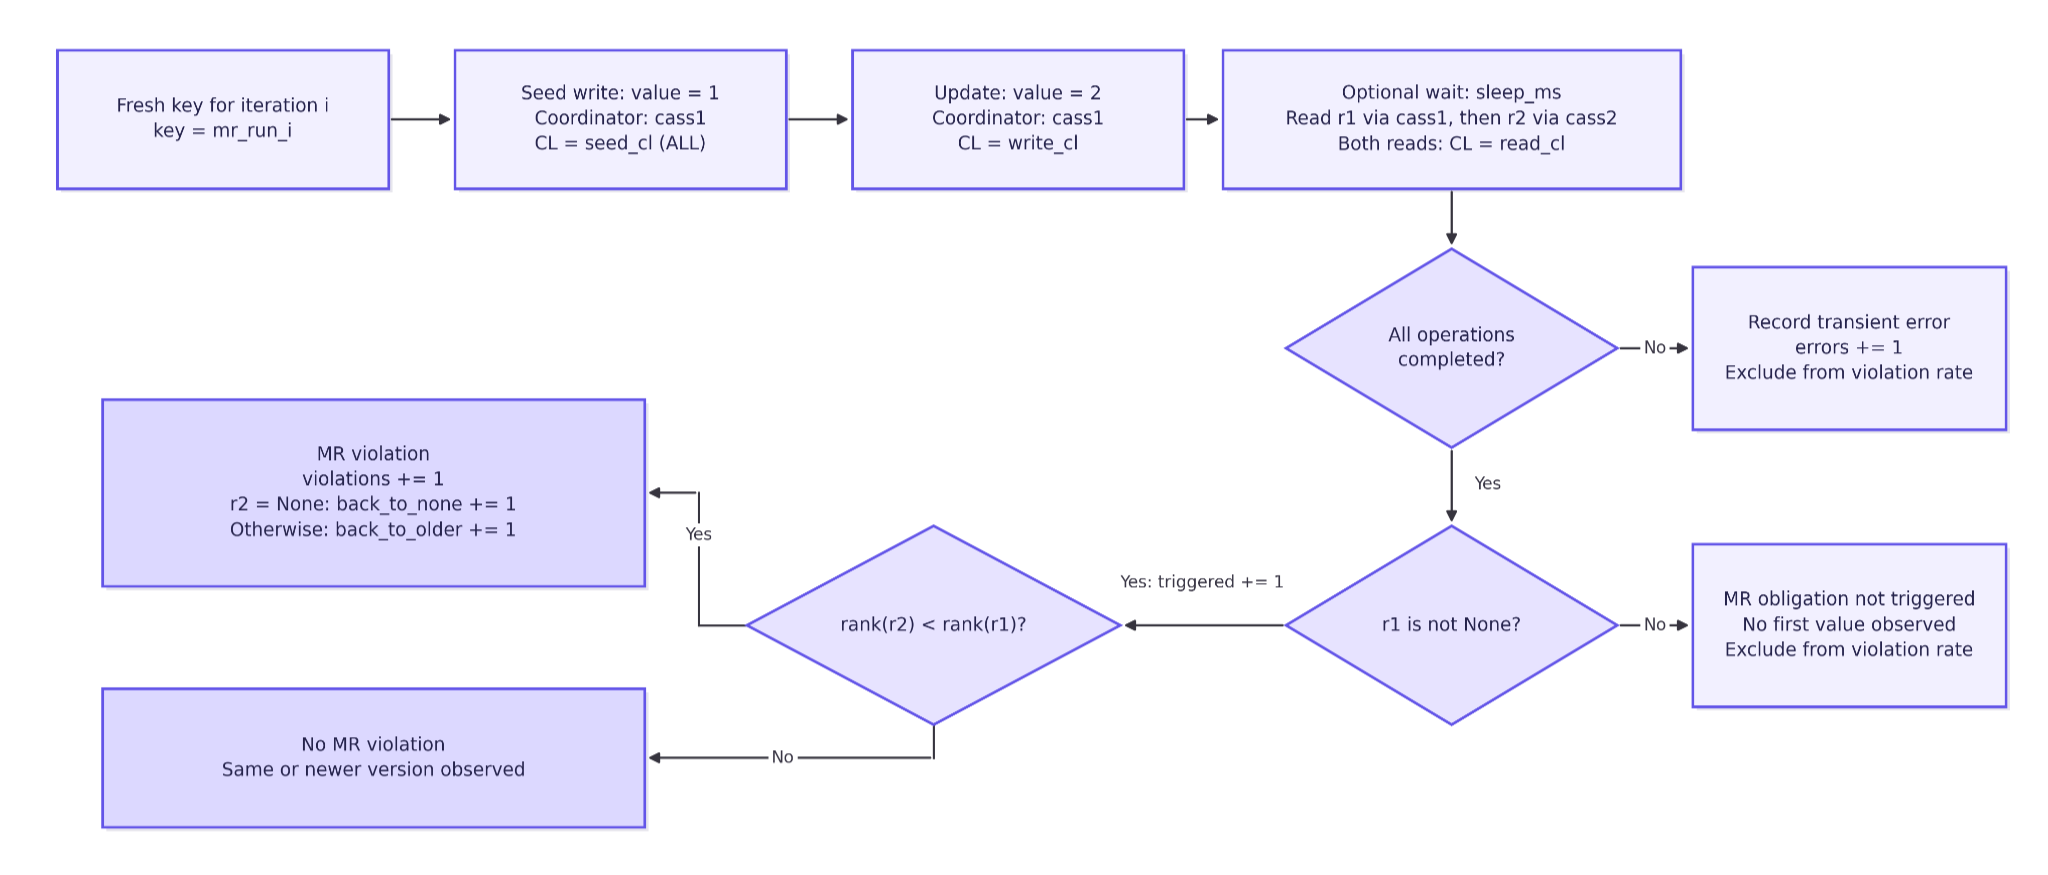
\includegraphics[width=\linewidth]{figures/mr_flow.png}
\caption{Monotonic-reads experimental workflow.}
\label{fig:mr-flow}
\end{figure}

The actual predicate is rank(r2) \textless{} rank(r1), where missing values have rank −1. Since the controlled values are version markers 1 and 2, a transition from 2 to 1 is a monotonic-read violation. Two reads returning 1 are stale relative to the update, but are not a monotonic-read violation: the client has not moved backwards.

For the completed update in this workload, write/read intersection provides a useful sufficient condition: W + R \textgreater{} RF. QUORUM--QUORUM satisfies 2 + 2 \textgreater{} 3, while ALL--ONE satisfies 3 + 1 \textgreater{} 3. This reasoning assumes the intended timestamp order, successful operations, and no competing later writes.

Read repair is relevant to weaker writes followed by quorum reads. Cassandra documents that read\_repair=`NONE' still reconciles returned replica data, but does not repair replicas or provide the general monotonic-quorum-read guarantee associated with blocking read repair. More details can be found here: \href{https://cassandra.apache.org/doc/latest/cassandra/managing/operating/read_repair.html}{Apache Cassandra read-repair documentation}

\subsubsection{Predicted Outcomes}\label{mr:predicted-outcomes}

{
\begin{table}[H]
\centering
\small
\renewcommand{\arraystretch}{1.15}
\caption{Predicted MR outcomes for the tested consistency-level combinations.}\label{tab:mr-2}
\begin{tabular}{@{}
  >{\RaggedRight\arraybackslash}p{(\linewidth - 4\tabcolsep) * \real{0.1600}}
  >{\RaggedRight\arraybackslash}p{(\linewidth - 4\tabcolsep) * \real{0.1600}}
  >{\RaggedRight\arraybackslash}p{(\linewidth - 4\tabcolsep) * \real{0.6800}}@{}}
\toprule\noalign{}
\begin{minipage}[b]{\linewidth}\RaggedRight
Write CL
\end{minipage} & \begin{minipage}[b]{\linewidth}\RaggedRight
Read CL
\end{minipage} & \begin{minipage}[b]{\linewidth}\RaggedRight
Expected Behavior
\end{minipage} \\
\midrule\noalign{}
ONE & ONE & Violations are possible and should become more frequent as delayed propagation outlasts the two client reads. \\
ONE & QUORUM & Violations are theoretically possible, but need not occur in this timing and routing arrangement. \\
QUORUM & QUORUM & No violations expected after the update succeeds, because each quorum intersects its acknowledgement set. \\
ALL & ONE & No violations expected after the update succeeds, because all replicas have acknowledged it. \\
\bottomrule
\end{tabular}
\end{table}
}

In particular, ONE--QUORUM does not satisfy strict write/read intersection: 1 + 2 = 3. If only replica A has value 2, a read involving A can return 2, while a later read involving only B and C can return 1 before propagation reaches them. This is a possible execution, not a prediction of a fixed violation probability. Replica selection should not be assumed uniformly random.

\subsubsection{Results and Analysis}\label{mr:actual-results-and-analysis}

\begin{figure}[H]
\centering
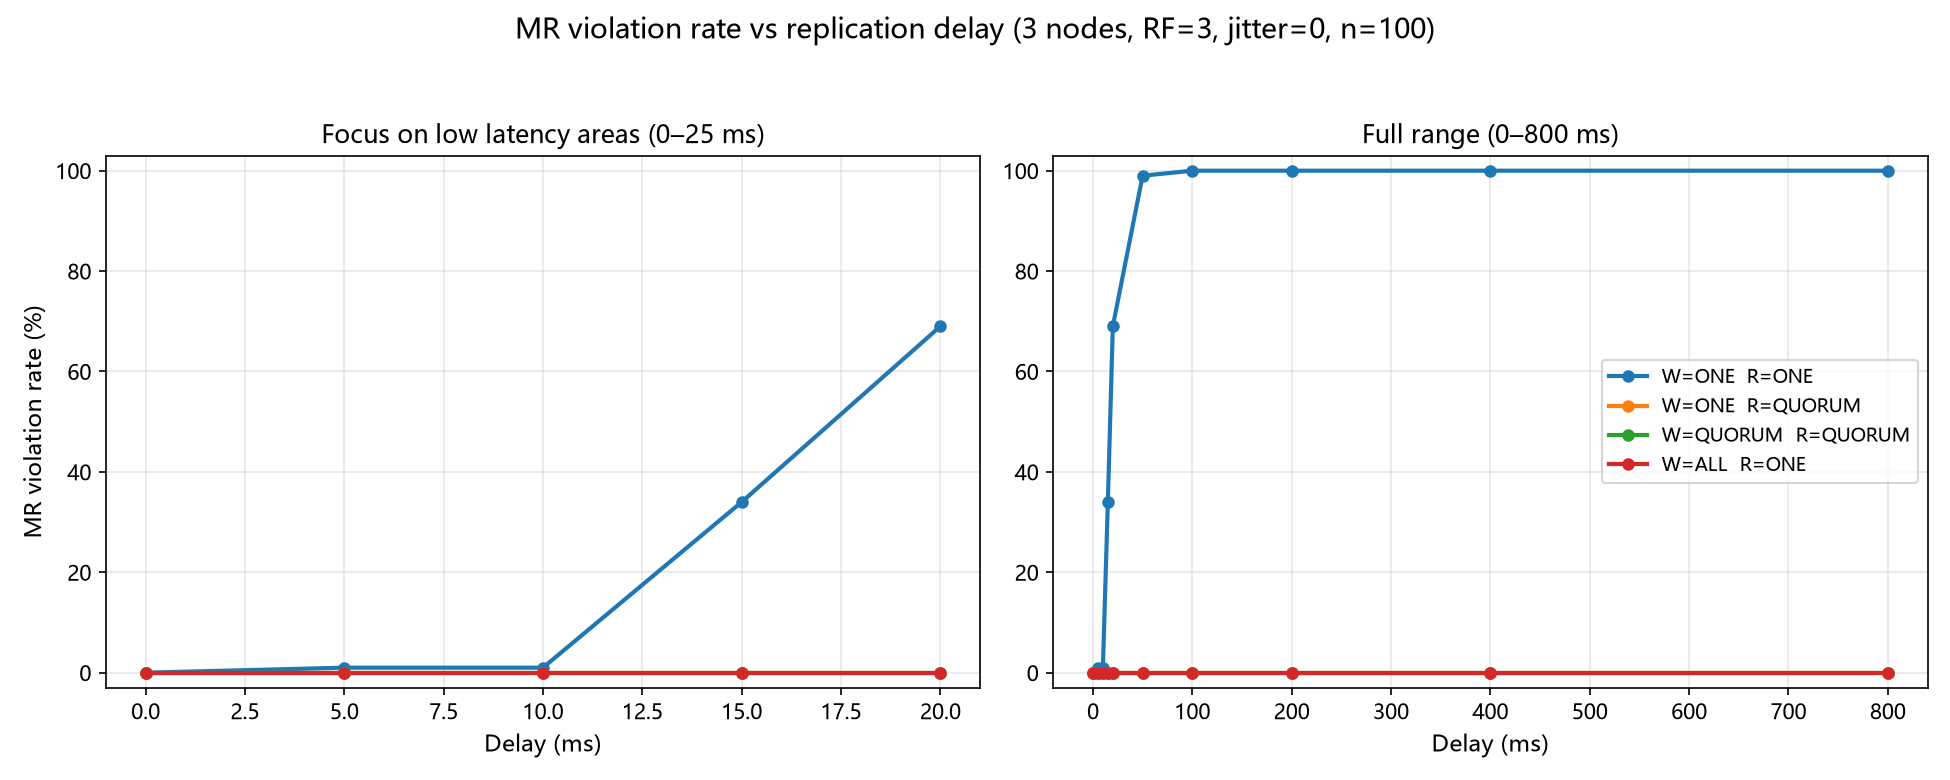
\includegraphics[width=\linewidth]{figures/mr_delay.png}
\caption{Monotonic-reads violation rate versus replication delay.}
\label{fig:mr-delay}
\end{figure}

The above plots demonstrate the violation rates vs different replication delays under different write consistency levels and read consistency levels. Detailed records and original data can be found in \href{https://github.com/LuweiChenbot/Cassandra-Lab/blob/main/results/mr_windows.csv}{monotonic-reads-results}. It is obvious that `ONE--ONE' exhibits a sharp increase between 10 and 50 ms and reaches 100\% at every tested delay of at least 100 ms. The remaining combinations have no observed violations throughout the whole delay range.

The partition rows in the \href{https://github.com/LuweiChenbot/Cassandra-Lab/blob/main/results/mr_windows.csv}{mr results} provide separate availability evidence. When node 3 is isolated and requests use nodes 1 and 2, ONE--ONE records 91/100 violations at delay = 100 ms and jitter = 50 ms; ONE--QUORUM and QUORUM--QUORUM record none. ALL--ONE has 100 operation errors and no valid samples. In the partition-labelled zero-delay run, the three available combinations record no violations, while ALL--ONE again fails every iteration. On the isolated node 3, only ONE--ONE completes the MR experiment, with no violations; combinations requiring a quorum or all replicas have no valid samples.

The ONE--ONE curve is consistent with a race between replica propagation and the client's read sequence. At short delays, the remote replica often receives the update before the second read. As the delay grows, the interval during which replicas hold different versions becomes longer, making a 2-to-1 observation more likely. The observed transition around 15--20 ms is specific to this environment and workload; it is not an intrinsic Cassandra threshold. Zero configured jitter also does not eliminate scheduling, processing, or transport variability.

The absence of ONE--QUORUM violations does not establish a consistency guarantee. A plausible explanation is that the first quorum read introduces an internode exchange, giving the outstanding write time to propagate before the second read. Replica selection and reconciliation can further reduce the opportunity to observe an older version. Because the same delay filter affects internode read traffic, increasing the configured delay can lengthen both propagation and the first read. These mechanisms are interpretations of the setup, not confirmed request-level traces. The supplied aggregate CSV cannot identify the exact replicas or message ordering responsible for the zero rate.

QUORUM--QUORUM and ALL--ONE match the expected intersection argument for this successful-write workload. Their stronger acknowledgement requirements prevent the particular stale-read sequence that ONE--ONE exposes. The partition results additionally show the availability cost: operations requiring unreachable replicas fail. Such failures must not be reported as successful consistency outcomes. Likewise, the isolated-node ONE--ONE result tests a single-node path, not migration between divergent replicas.

\paragraph{Detailed Results Across Topologies}\label{mr:detailed-results-across-topologies}

Each table entry below gives violations / valid iterations; iteration error rate. Every configuration was attempted 100 times. Unlike the plot, these tables include unavailable configurations.

{
\begin{table}[H]
\centering
\small
\renewcommand{\arraystretch}{1.15}
\caption{MR results across topologies: violations / valid iterations; iteration error rate.}\label{tab:mr-3}
\begin{tabular}{@{}
  >{\RaggedRight\arraybackslash}p{(\linewidth - 10\tabcolsep) * \real{0.1667}}
  >{\RaggedRight\arraybackslash}p{(\linewidth - 10\tabcolsep) * \real{0.1667}}
  >{\RaggedRight\arraybackslash}p{(\linewidth - 10\tabcolsep) * \real{0.1667}}
  >{\RaggedRight\arraybackslash}p{(\linewidth - 10\tabcolsep) * \real{0.1667}}
  >{\RaggedRight\arraybackslash}p{(\linewidth - 10\tabcolsep) * \real{0.1667}}
  >{\RaggedRight\arraybackslash}p{(\linewidth - 10\tabcolsep) * \real{0.1667}}@{}}
\toprule\noalign{}
\begin{minipage}[b]{\linewidth}\RaggedRight
Topology
\end{minipage} & \begin{minipage}[b]{\linewidth}\RaggedRight
Delay/\allowbreak Jitter\_ms
\end{minipage} & \begin{minipage}[b]{\linewidth}\RaggedRight
ONE-ONE
\end{minipage} & \begin{minipage}[b]{\linewidth}\RaggedRight
ONE-QUORUM
\end{minipage} & \begin{minipage}[b]{\linewidth}\RaggedRight
QUORUM-QUORUM
\end{minipage} & \begin{minipage}[b]{\linewidth}\RaggedRight
ALL-ONE
\end{minipage} \\
\midrule\noalign{}
normal, initial baseline & 0/0 & 0/100; 0\% & 0/100; 0\% & 0/100; 0\% & 0/100; 0\% \\
normal & 100/50 & 88/100; 0\% & 0/100; 0\% & 0/100; 0\% & 0/100; 0\% \\
partition majority & 0/0 & 0/100; 0\% & 0/100; 0\% & 0/100; 0\% & N/A; 100\% \\
partition majority & 100/50 & 91/100; 0\% & 0/100; 0\% & 0/100; 0\% & N/A; 100\% \\
partition minority & 0/0 & 0/100; 0\% & N/A; 100\% & N/A; 100\% & N/A; 100\% \\
partition minority & 100/50 & 0/100; 0\% & N/A; 100\% & N/A; 100\% & N/A; 100\% \\
\bottomrule
\end{tabular}
\end{table}
}

Normal topology: with all nodes reachable, all four configurations complete every iteration. At 100/50 ms, ONE--ONE exposes a stale second read in 88 trials. The other configurations have no measured violations. Thus reachability alone does not ensure that a client changing coordinators sees monotonically newer data.

Majority partition: the seed write is reduced to QUORUM so that both reachable replicas can be initialized without requiring node 3. Under ONE--ONE, the update may complete on one majority replica while the other still holds the seed value. The partition therefore does not eliminate the divergence window within the majority: 91\% of trials violate MR at 100/50 ms, compared with 0\% at 0/0 ms.

ONE--QUORUM deserves a different explanation here than in the normal topology. During the stable tested partition, a successful quorum read must obtain both reachable replicas, nodes 1 and 2. There is no alternative successful quorum consisting of two other stale replicas. The completed ONE write is represented on at least one member of this pair, so the read can reconcile against that version. The observed zero rate therefore has a stronger workload-specific explanation than the normal three-node ONE--QUORUM zero. This does not convert ONE--QUORUM into a universal session guarantee during arbitrary membership changes or partition healing.

QUORUM--QUORUM also completes with no violations because both reachable replicas acknowledge the update. ALL--ONE cannot complete its update with node 3 isolated; the observed error rate is 100\%. The 91\% majority result and 88\% normal result differ by only three trials out of 100 each. These runs do not establish that partitioning intrinsically increases MR violations; both demonstrate a large stale-read window under weak consistency.

Minority partition\textbf{:} all MR operations use node 3, and the seed CL is ONE. ONE--ONE can complete locally and records no backwards reads. This outcome is expected for the specific same-node overwrite-and-read sequence. It does not show that node 3 is synchronized with the majority, or that a client migrating between the two sides would preserve MR. Each iteration uses its own key, so these tests also do not measure simultaneous conflicting writes to the same key across both partitions.

For ONE--QUORUM on the minority, the local update can succeed but the quorum read cannot obtain a second response. For QUORUM--QUORUM and ALL--ONE, the selected update CL already requires unreachable replicas. This explains why all three configurations have 100\% iteration errors, while only ONE--ONE produces valid consistency observations.

\paragraph{Additional Delay, Jitter, and Read-Path Probes}\label{mr:additional-delay-jitter-and-read-path-probes}

The following table includes all 11 supplementary MR rows. Every row has zero operation errors, so attempted and valid sample counts coincide.

{
\begin{table}[H]
\centering
\small
\renewcommand{\arraystretch}{1.15}
\caption{Supplementary MR experiments with different delays, jitter, and read paths.}\label{tab:mr-4}
\begin{tabular}{@{}
  >{\RaggedRight\arraybackslash}p{(\linewidth - 8\tabcolsep) * \real{0.2000}}
  >{\RaggedRight\arraybackslash}p{(\linewidth - 8\tabcolsep) * \real{0.2000}}
  >{\RaggedRight\arraybackslash}p{(\linewidth - 8\tabcolsep) * \real{0.2000}}
  >{\RaggedRight\arraybackslash}p{(\linewidth - 8\tabcolsep) * \real{0.2000}}
  >{\RaggedRight\arraybackslash}p{(\linewidth - 8\tabcolsep) * \real{0.2000}}@{}}
\toprule\noalign{}
\begin{minipage}[b]{\linewidth}\RaggedRight
Delay/\allowbreak Jitter\_ms
\end{minipage} & \begin{minipage}[b]{\linewidth}\RaggedRight
W-R
\end{minipage} & \begin{minipage}[b]{\linewidth}\RaggedRight
Read Path
\end{minipage} & \begin{minipage}[b]{\linewidth}\RaggedRight
Violation Rate
\end{minipage} & \begin{minipage}[b]{\linewidth}\RaggedRight
Valid Iterations
\end{minipage} \\
\midrule\noalign{}
10/10 & ONE-QUORUM & 1→2 & 0\% & 200 \\
20/10 & ONE-QUORUM & 1→2 & 0\% & 200 \\
50/50 & ONE-QUORUM & 1→2 & 0\% & 200 \\
50/50 & ONE-QUORUM & 2→2 & 0\% & 200 \\
50/50 & ONE-ONE & 1→2 & 63.5\% & 200 \\
50/50 & ONE-ONE & 2→2 & 0\% & 200 \\
50/50 & ONE-QUORUM & 1→3 & 0\% & 200 \\
50/50 & ONE-ONE & 1→3 & 62.5\% & 200 \\
100/50 & ONE-QUORUM & 1→2 & 0\% & 200 \\
100/50 & ONE-ONE & 1→2 & 93\% & 200 \\
100/50 & ONE-ONE & 2→2 & 0\% & 200 \\
\bottomrule
\end{tabular}
\end{table}
}

Effect of changing the read path: at 50/50 ms, ONE--ONE yields nearly identical rates on paths 1 → 2 and 1 → 3: 63.5\% and 62.5\%. The effect is therefore observed with two different second-read coordinators, rather than only node 2. In contrast, 2 → 2 produces no violations at either 50/50 or 100/50 ms. Reusing the same coordinator removes the explicit coordinator switch that creates the main test's backwards-read opportunity. It does not establish that all reads were fresh: both could return 1 without violating MR. Coordinator pinning also does not prove an identical replica set for every read.

Effect of jitter: at base delay 50 ms, the deterministic 50/0 sweep produces 99/100 violations, whereas the 50/50 path-1 → 2 probe produces 127/200 (63.5\%). At base delay 100 ms, the 100/0 sweep produces 100/100 violations, while separate 100/50 runs produce 88/100 and 186/200 (93\%). A plausible explanation is that variable delay allows some updates to propagate earlier, shortening the stale interval for those trials; other packets are delayed longer. This is an interpretation of observed timing-sensitive outcomes. Different sample sizes and sequentially collected runs prevent a precise causal estimate of jitter's independent effect, and the results do not imply that jitter always improves consistency.

Effect of increasing base delay at fixed jitter: for ONE--ONE on path 1 → 2, increasing base delay from 50 to 100 ms while keeping jitter at 50 ms raises the measured rate from 63.5\% to 93\% in the two 200-trial probes. This agrees with the deterministic sweep's evidence that longer propagation windows increase the chance of a stale second read.

Persistent zero results under quorum reads: all six supplementary ONE--QUORUM runs, totalling 1,200 valid trials across different settings and paths, record zero violations. The supplementary data strengthen the observation that this implementation rarely or never exposes the theoretically permitted ONE--QUORUM anomaly under these tested schedules. They do not identify a formal guarantee. Unlike the majority partition, the normal topology still permits different quorum pairs; response timing, selected replicas, and propagation during the first read remain plausible explanations.

\paragraph{Conclution}\label{mr:conclution}

The combined evidence supports three distinct statements. First, switching read coordinators under ONE--ONE exposes clear backwards reads when propagation is slow. Second, the particular same-coordinator probes and normal ONE--QUORUM runs show no backwards reads, but their zero rates must be interpreted in light of path and timing. Third, partitions change which requests can finish: majority quorums remain available, while the isolated minority can serve only local ONE requests in the MR test.

A single pooled MR percentage would mix these different questions. For example, grouping all partition rows together would combine a majority path with 91\% violations and a minority same-node path with 0\%, as well as configurations producing no valid samples. Reporting them separately preserves both the consistency and availability findings.

\subsection{Monotonic-writes consistency}\label{mw:monotonic-writes-consistency}

\subsubsection{Definition}\label{mw:definition}

Monotonic-writes (MW) consistency guarantees that writes issued by the same client are applied in the order the client issued them. For example, suppose a client first writes \(x=1\) and then updates it to \(x=2\). A replica applying both writes should apply the first before the second, even if the requests pass through different coordinators. If it applies them in the reverse order, the earlier write may overwrite the later update, violating MW consistency.

\subsubsection{Experimental Design}\label{mw:experimental-design}

Monotonic writes concern preservation of a client's write order. This experiment examines a specific observable consequence: after sequential overwrites W1 and W2 of the same key, does the reconciled value reflect the later operation W2?

For each iteration, the client writes value 1 through node 2 and waits for completion, then writes value 2 through node 3. Both writes use the selected write consistency level. Verification is performed through node 1 using verify\_cl=ALL in the normal topology. The query returns the value, writer identifier, and WRITETIME(value).

Two modes separate ordinary execution from a deliberately inverted timestamp order: Natural mode: both writes use ordinary driver-generated timestamps. Skew mode: explicit CQL timestamps assign W1 the timestamp base + 500000 microseconds and W2 the timestamp base. Thus the first operation receives a timestamp 500 ms greater than the second.

The skew mode models client-supplied timestamp inversion. It does not modify or directly measure clock differences between Cassandra coordinators.

\subsubsection{Principle and Key Implementation}\label{mw:principle-and-key-implementation}

Cassandra's timestamp-based last-write-wins reconciliation makes the relative timestamps decisive for these competing cell values. Write consistency determines how many acknowledgements are required; it does not change the explicit timestamps used by this experiment.

\begin{figure}[H]
\centering
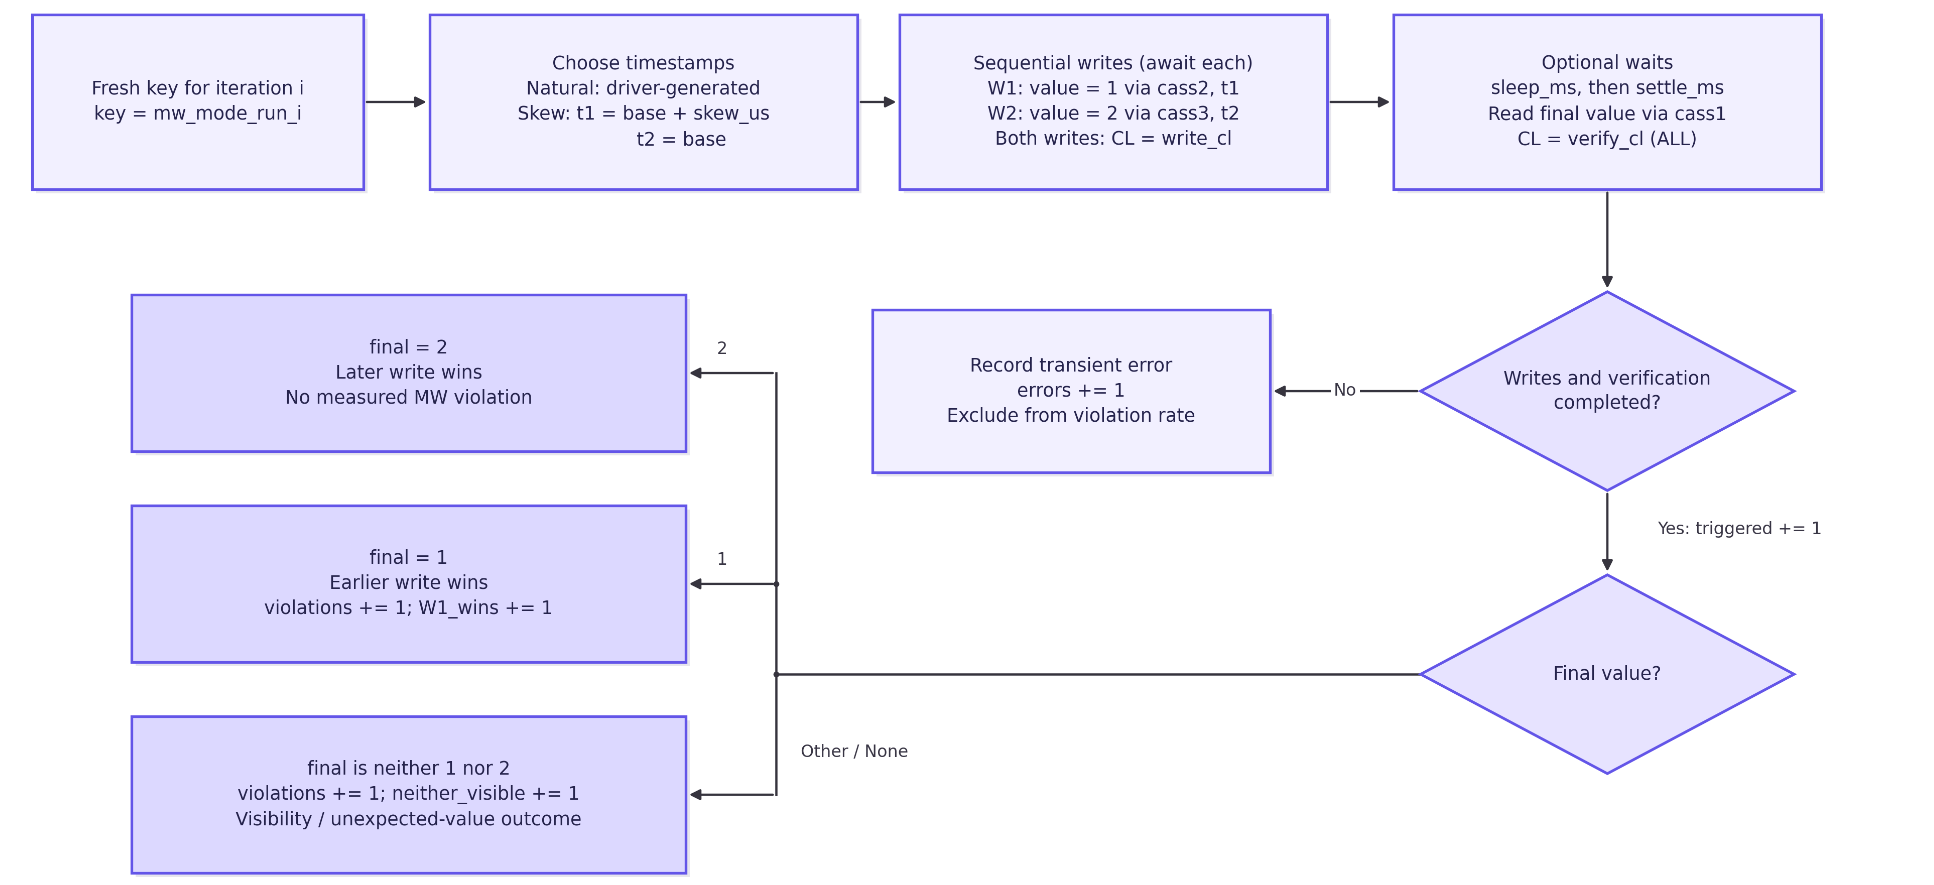
\includegraphics[width=\linewidth]{figures/mw_flow.png}
\caption{Monotonic-writes experimental workflow.}
\label{fig:mw-flow}
\end{figure}

The explicit-timestamp path uses INSERT \ldots{} USING TIMESTAMP. Verification uses SELECT value, writer, WRITETIME(value) \ldots. An ALL read reconciles responses from all replicas and reduces the risk of classifying a read from an uninformed replica as a write-order failure. It does not, by itself, prove that every replica has physically converged or reveal the order in which each replica applied mutations.

Although the matrix and plot retain read\_cl labels, the MW script does not use that parameter for verification. In the normal sweep every verification read uses ALL. Consequently, ONE--ONE and ONE--QUORUM are repeated tests with the same effective write and verification levels.

The driver documentation specifies a default monotonic timestamp generator per Cluster instance. Here, common.py creates a separate Cluster for each pinned node, so there is no explicitly shared generator across the two write connections. Increasing timestamps are expected under the observed sequential execution and stable client clock, but are not guaranteed across these separate generators merely by their individual monotonicity. \href{https://docs.datastax.com/en/developer/python-driver/3.29/api/cassandra/cluster/index.html}{DataStax Python driver documentation}.

\subsubsection{Predicted Outcomes}\label{mw:predicted-outcomes}

In natural mode, if W2 receives a greater timestamp than W1, value 2 should win reconciliation at every tested write consistency level. Delaying replication alone should not change that winner.

In skew mode, W1 has the greater timestamp by construction, despite W2 being issued later. Value 1 should therefore win, producing a 100\% measured violation rate under the script's final != 2 criterion. Raising write consistency to QUORUM or ALL cannot reverse the supplied timestamp order.

{
\begin{table}[H]
\centering
\small
\renewcommand{\arraystretch}{1.15}
\caption{Predicted MW outcomes under natural and inverted timestamp ordering.}\label{tab:mw-1}
\begin{tabular}{@{}
  >{\RaggedRight\arraybackslash}p{(\linewidth - 6\tabcolsep) * \real{0.2500}}
  >{\RaggedRight\arraybackslash}p{(\linewidth - 6\tabcolsep) * \real{0.2500}}
  >{\RaggedRight\arraybackslash}p{(\linewidth - 6\tabcolsep) * \real{0.2500}}
  >{\RaggedRight\arraybackslash}p{(\linewidth - 6\tabcolsep) * \real{0.2500}}@{}}
\toprule\noalign{}
\begin{minipage}[b]{\linewidth}\RaggedRight
Mode
\end{minipage} & \begin{minipage}[b]{\linewidth}\RaggedRight
Timestamp Relationship
\end{minipage} & \begin{minipage}[b]{\linewidth}\RaggedRight
Expected Winning Value
\end{minipage} & \begin{minipage}[b]{\linewidth}\RaggedRight
Expected Measured Rate
\end{minipage} \\
\midrule\noalign{}
natural & normally t2 \textgreater{} t1 & 2 & 0\% \\
skew & t1 = t2 + 500000 \(\mu\)s & 1 & 100\% \\
\bottomrule
\end{tabular}
\end{table}
}

\subsubsection{Results and Analysis}\label{mw:actual-results-and-analysis}

Across all ten delay settings, each retained mode/configuration row contains 100 valid iterations and zero operation errors.

{
\begin{table}[H]
\centering
\small
\renewcommand{\arraystretch}{1.15}
\caption{MW delay-sweep outcomes among successful verification reads.}\label{tab:mw-2}
\begin{tabular}{@{}llll@{}}
\toprule\noalign{}
W-R & Actual Verification CL & Natural Mode & Skew Mode \\
\midrule\noalign{}
ONE-ONE & ALL & 0\% at every delay & 100\% at every delay \\
ONE-QUORUM & ALL & 0\% at every delay & 100\% at every delay \\
QUORUM-QUORUM & ALL & 0\% at every delay & 100\% at every delay \\
ALL-ONE & ALL & 0\% at every delay & 100\% at every delay \\
\bottomrule
\end{tabular}
\end{table}
}

Detailed records can be found in \href{https://github.com/LuweiChenbot/Cassandra-Lab/blob/main/results/mw_windows.csv}{monotonic-write-records}. The two modes separate propagation delay from timestamp ordering. In natural mode, delayed delivery does not prevent the later write from winning reconciliation. In skew mode, the earlier write consistently wins because its assigned timestamp is larger. The result remains unchanged even when all replicas acknowledge both writes: stronger acknowledgements do not repair an inversion between application order and timestamp order.

The 500 ms skew is a difference between two assigned timestamps, not a waiting period. Therefore, increasing network delay beyond 500 ms does not remove the inversion; t1 remains greater than t2 regardless of elapsed execution time.

The main interpretive limitation is the measurement itself. The script tests whether the later application overwrite wins a reconciled read. It does not instrument per-replica mutation histories, enforce cross-key dependencies, or establish the full formal monotonic-writes property. The most precise conclusion is that natural execution preserved the intended overwrite result in all tested trials, while explicit timestamp inversion defeated that result at every tested write consistency level. The reported MW violation rate should be accompanied by this operational definition.

These findings indicate that preserving application write order requires attention to timestamp generation across the logical client session, including multiple connections or client instances. Raising consistency levels addresses acknowledgement and visibility requirements, but is insufficient to make timestamp-based conflict resolution follow application order when the timestamps themselves are inverted.

\paragraph{Detailed MW Results Across Topologies}\label{mw:detailed-mw-results-across-topologies}

The table below applies separately to both recorded partition/network settings, 0/0 ms and 100/50 ms. Normal has complete matrices at these settings as well as the ten-point zero-jitter sweep. Each natural or skew entry represents 100 attempted iterations per setting and row.

{
\begin{table}[H]
\centering
\small
\renewcommand{\arraystretch}{1.15}
\caption{MW results across topologies, applied separately at 0/0 ms and 100/50 ms delay/jitter.}\label{tab:mw-3}
\begin{tabular}{@{}
  >{\RaggedRight\arraybackslash}p{(\linewidth - 10\tabcolsep) * \real{0.1667}}
  >{\RaggedRight\arraybackslash}p{(\linewidth - 10\tabcolsep) * \real{0.1667}}
  >{\RaggedRight\arraybackslash}p{(\linewidth - 10\tabcolsep) * \real{0.1667}}
  >{\RaggedRight\arraybackslash}p{(\linewidth - 10\tabcolsep) * \real{0.1667}}
  >{\RaggedRight\arraybackslash}p{(\linewidth - 10\tabcolsep) * \real{0.1667}}
  >{\RaggedRight\arraybackslash}p{(\linewidth - 10\tabcolsep) * \real{0.1667}}@{}}
\toprule\noalign{}
\begin{minipage}[b]{\linewidth}\RaggedRight
Topology
\end{minipage} & \begin{minipage}[b]{\linewidth}\RaggedRight
W-R
\end{minipage} & \begin{minipage}[b]{\linewidth}\RaggedRight
Actual verification CL
\end{minipage} & \begin{minipage}[b]{\linewidth}\RaggedRight
Natural: violations/valid
\end{minipage} & \begin{minipage}[b]{\linewidth}\RaggedRight
Skew: violations/valid
\end{minipage} & \begin{minipage}[b]{\linewidth}\RaggedRight
Iteration error rate
\end{minipage} \\
\midrule\noalign{}
normal & ONE-ONE & ALL & 0/100 & 100/100 & 0\% \\
normal & ONE-QUORUM & ALL & 0/100 & 100/100 & 0\% \\
normal & QUORUM-QUORUM & ALL & 0/100 & 100/100 & 0\% \\
normal & ALL-ONE & ALL & 0/100 & 100/100 & 0\% \\
partition majority & ONE-ONE & QUORUM & 0/100 & 100/100 & 0\% \\
partition majority & ONE-QUORUM & QUORUM & 0/100 & 100/100 & 0\% \\
partition majority & QUORUM-QUORUM & QUORUM & 0/100 & 100/100 & 0\% \\
partition majority & ALL-ONE & QUORUM & N/A & N/A & 100\% \\
partition minority & ONE-ONE & ONE & 0/100 & 100/100 & 0\% \\
partition minority & ONE-QUORUM & ONE & 0/100 & 100/100 & 0\% \\
partition minority & QUORUM-QUORUM & ONE & N/A & N/A & 100\% \\
partition minority & ALL-ONE & ONE & N/A & N/A & 100\% \\
\bottomrule
\end{tabular}
\end{table}
}

Normal topology: delay changes delivery, while the assigned timestamps determine the observed winner. All writes and ALL verification reads complete at every supplied normal setting. Natural mode always returns the intended later value. Skew mode always preserves W1. The 100/50 ms jittered matrix agrees with the deterministic sweep. Thus neither zero jitter nor fixed packet timing is necessary for the observed timestamp-inversion outcome. These files contain outcome counts, not request-latency distributions, so they cannot quantify the performance cost of stronger CLs or larger delays.

Majority partition: verification is scoped to the two reachable replicas. W1 is sent through node 1 and W2 through node 2, with verification through node 1 at QUORUM. Both writes at ONE or QUORUM can finish within this component. The verification quorum covers both reachable replicas, and the matrix adds a settling interval. Natural mode returns 2; skew mode returns 1 at both 0/0 and 100/50 ms. ALL writes cannot obtain three acknowledgements, leaving no valid order check. Successful majority verification does not show that isolated node 3 has converged; it reports the reconciled outcome available within the majority.

Minority partition: timestamp inversion occurs even without changing nodes. W1, W2, and verification all use node 3. With W=ONE, natural mode returns 2, but skew mode still returns 1 in every trial. This is particularly informative: the undesired overwrite result can arise entirely on one replica when the application supplies inverted timestamps. Neither cross-node delivery reordering nor communication with another replica is necessary to produce it. Network partitioning determines which CLs remain usable, while the explicit timestamp order determines which of the two values wins locally.

The nominal ONE--QUORUM minority row completes because the MW script never executes a read at its read\_cl label: it uses verify\_cl=ONE. This explains the apparent contrast with MR, where ONE--QUORUM fails on the minority because an actual quorum read is attempted. Comparing the two models solely by plot legends would therefore give a misleading availability conclusion.

Unavailable configurations. Both modes fail at ALL on the majority and at QUORUM or ALL on the minority. A zero stored violation count in these rows means no successful verification was available, not that timestamp skew was harmless. The correct outcome is ``ordering result unavailable; iteration error rate 100\%.''

\paragraph{Full-Dataset Accounting and Scope of the MW Claim}\label{mw:full-dataset-accounting-and-scope-of-the-mw-claim}

The following totals retain every supplied row, including repeated zero-delay normal baselines. They are an inventory of evidence, not a balanced estimate across operating conditions.

{
\begin{table}[H]
\centering
\small
\renewcommand{\arraystretch}{1.15}
\caption{Full-dataset MW accounting by topology and timestamp mode.}\label{tab:mw-4}
\begin{tabular}{@{}
  >{\RaggedRight\arraybackslash}p{(\linewidth - 8\tabcolsep) * \real{0.2000}}
  >{\RaggedRight\arraybackslash}p{(\linewidth - 8\tabcolsep) * \real{0.2000}}
  >{\RaggedRight\arraybackslash}p{(\linewidth - 8\tabcolsep) * \real{0.2000}}
  >{\RaggedRight\arraybackslash}p{(\linewidth - 8\tabcolsep) * \real{0.2000}}
  >{\RaggedRight\arraybackslash}p{(\linewidth - 8\tabcolsep) * \real{0.2000}}@{}}
\toprule\noalign{}
\begin{minipage}[b]{\linewidth}\RaggedRight
Topology
\end{minipage} & \begin{minipage}[b]{\linewidth}\RaggedRight
Mode
\end{minipage} & \begin{minipage}[b]{\linewidth}\RaggedRight
Attempted iterations
\end{minipage} & \begin{minipage}[b]{\linewidth}\RaggedRight
Valid iterations
\end{minipage} & \begin{minipage}[b]{\linewidth}\RaggedRight
Measured violations
\end{minipage} \\
\midrule\noalign{}
normal & natural & 4800 & 4800 & 0 \\
normal & skew & 4800 & 4800 & 4800 \\
partition majority & natural & 800 & 600 & 0 \\
partition majority & skew & 800 & 600 & 600 \\
partition minority & natural & 800 & 400 & 0 \\
partition minority & skew & 800 & 400 & 400 \\
\bottomrule
\end{tabular}
\end{table}
}

Across all settings, natural mode has 0/5,800 measured violations among valid iterations, while skew mode has 5,800/5,800. Each mode also has 600 unavailable iterations. The 4,000-trial figures reported for the sweep refer only to its retained ten-delay subset and should not be confused with these whole-file totals.

The decisive comparison is conditional on successful verification: natural and skew modes yield opposite winners under every available tested configuration. The minority experiment shows that timestamp inversion is sufficient even locally; the normal ALL-write experiment shows that acknowledging every replica does not correct it. Together, these results substantiate a failure to preserve the application's intended overwrite order under inverted timestamps. They do not directly observe every replica's mutation order or establish a complete formal test of monotonic writes across multiple keys.

The full dataset consequently distinguishes three experimentally different effects: replication timing influences the opportunity for backwards reads; network reachability determines whether selected CLs can complete; and supplied timestamp order controls the winning overwrite in the MW test. Keeping these dimensions separate explains the observed curves, the majority/minority asymmetry, and the apparently conflicting zero and 100\% results.

\subsection{Writes-follow-reads Consistency}\label{wfr:writes-follow-reads-consistency}

\subsubsection{Definition}\label{wfr:definition}

Writes-follow-reads (WFR) consistency requires a write that follows a read by the same client to be performed on the same or a more recent version than the one previously read. For example, if a client reads version 2 and then submits an update based on it, the system should preserve the dependency between the observed version and the subsequent write.

Our experiment examines an observable consequence of this dependency: whether a read-dependent update survives Cassandra's timestamp-based reconciliation. As in the MW experiment, the final winning value is an operational indicator, not a direct observation of the order in which every replica applies mutations.

\subsubsection{Experimental Design}\label{wfr:experimental-design}

Each iteration uses a fresh key. A setup write $W_a$ first stores $x=1$, followed by a preceding write $W_b$ that stores $x=2$. The client then reads the key and issues a dependent write $x=r+10$, where $r$ is the observed value. A final verification read identifies the winning version. The coordinator paths and setup and verification consistency levels vary with the topology, as specified in Table~\ref{tab:wfr-topology}.

If the client reads $r=2$, it has observed $W_b$, and the dependent write stores $x=12$. This establishes the dependency tested by the experiment. A final value of 12 indicates that the dependent update was preserved; a final value of 2 indicates that the preceding write remained the winner despite the later dependent update. If the client reads $r=1$, the trial is recorded as a stale read and excluded from the violation rate for the dependency on $W_b$.

Two modes are used. In natural mode, writes use ordinary driver-generated timestamps, and $W_b$ uses the selected write CL. In skew mode, $W_b$ receives a future-dated timestamp and uses the verification CL listed in Table~\ref{tab:wfr-topology}, establishing its visibility within the participating component before the trigger read. In both modes, the trigger read uses the selected read CL, while the dependent write uses the selected write CL and a driver-generated timestamp. The original scenario matrix used a five-second timestamp offset and recorded whether it was sufficient to produce the intended inversion. Thus, the modes differ in both timestamp assignment and the CL used for $W_b$; their trigger rates should not be interpreted as a comparison that changes timestamps alone.

The scenario matrix contains 64 configurations: two delay/jitter settings, four operational scenarios, four write/read CL combinations, and two modes. Each configuration has 100 attempted iterations. The operational scenarios are normal operation, single-node failure, majority partition, and minority partition; the network settings are 0/0 ms and 100/50 ms delay/jitter.

\begin{table}[H]
\centering
\small
\renewcommand{\arraystretch}{1.15}
\caption{WFR setup and verification configurations by topology. In the coordinator path, node numbers denote cass1, cass2, and cass3; the order is $W_a/W_b$, trigger read, dependent write, and verification read.}
\label{tab:wfr-topology}
\begin{tabular}{@{}
>{\RaggedRight\arraybackslash}p{(\linewidth - 8\tabcolsep) * \real{0.24}}
>{\RaggedRight\arraybackslash}p{(\linewidth - 8\tabcolsep) * \real{0.14}}
>{\RaggedRight\arraybackslash}p{(\linewidth - 8\tabcolsep) * \real{0.17}}
>{\RaggedRight\arraybackslash}p{(\linewidth - 8\tabcolsep) * \real{0.29}}
>{\RaggedRight\arraybackslash}p{(\linewidth - 8\tabcolsep) * \real{0.16}}@{}}
\toprule
Scenario & Setup CL & Verification CL & Coordinator path & Settle time (ms) \\
\midrule
Normal & ALL & ALL & $1\to2\to3\to1$ & 0 \\
Node failure & QUORUM & QUORUM & $1\to2\to1\to1$ & 1000 \\
Majority partition & QUORUM & QUORUM & $1\to2\to1\to1$ & 1000 \\
Minority partition & ONE & ONE & $3\to3\to3\to3$ & 1000 \\
\bottomrule
\end{tabular}
\end{table}

No additional client-side sleep is inserted between $W_b$ and the trigger read. The settling interval in Table~\ref{tab:wfr-topology} occurs only after the dependent write and before verification. Verification covers all three replicas in the normal topology, the two reachable replicas under node failure or majority partition, and only cass3 in the minority partition. The fixed settling interval is not itself proof of convergence, and partition-local verification does not establish convergence across the partition.

The additional delay plots present natural and skew results at 0, 5, 10, 20, and 50 ms with zero configured jitter. These scanning results are discussed separately from the scenario matrix.

\begin{figure}[H]
\centering
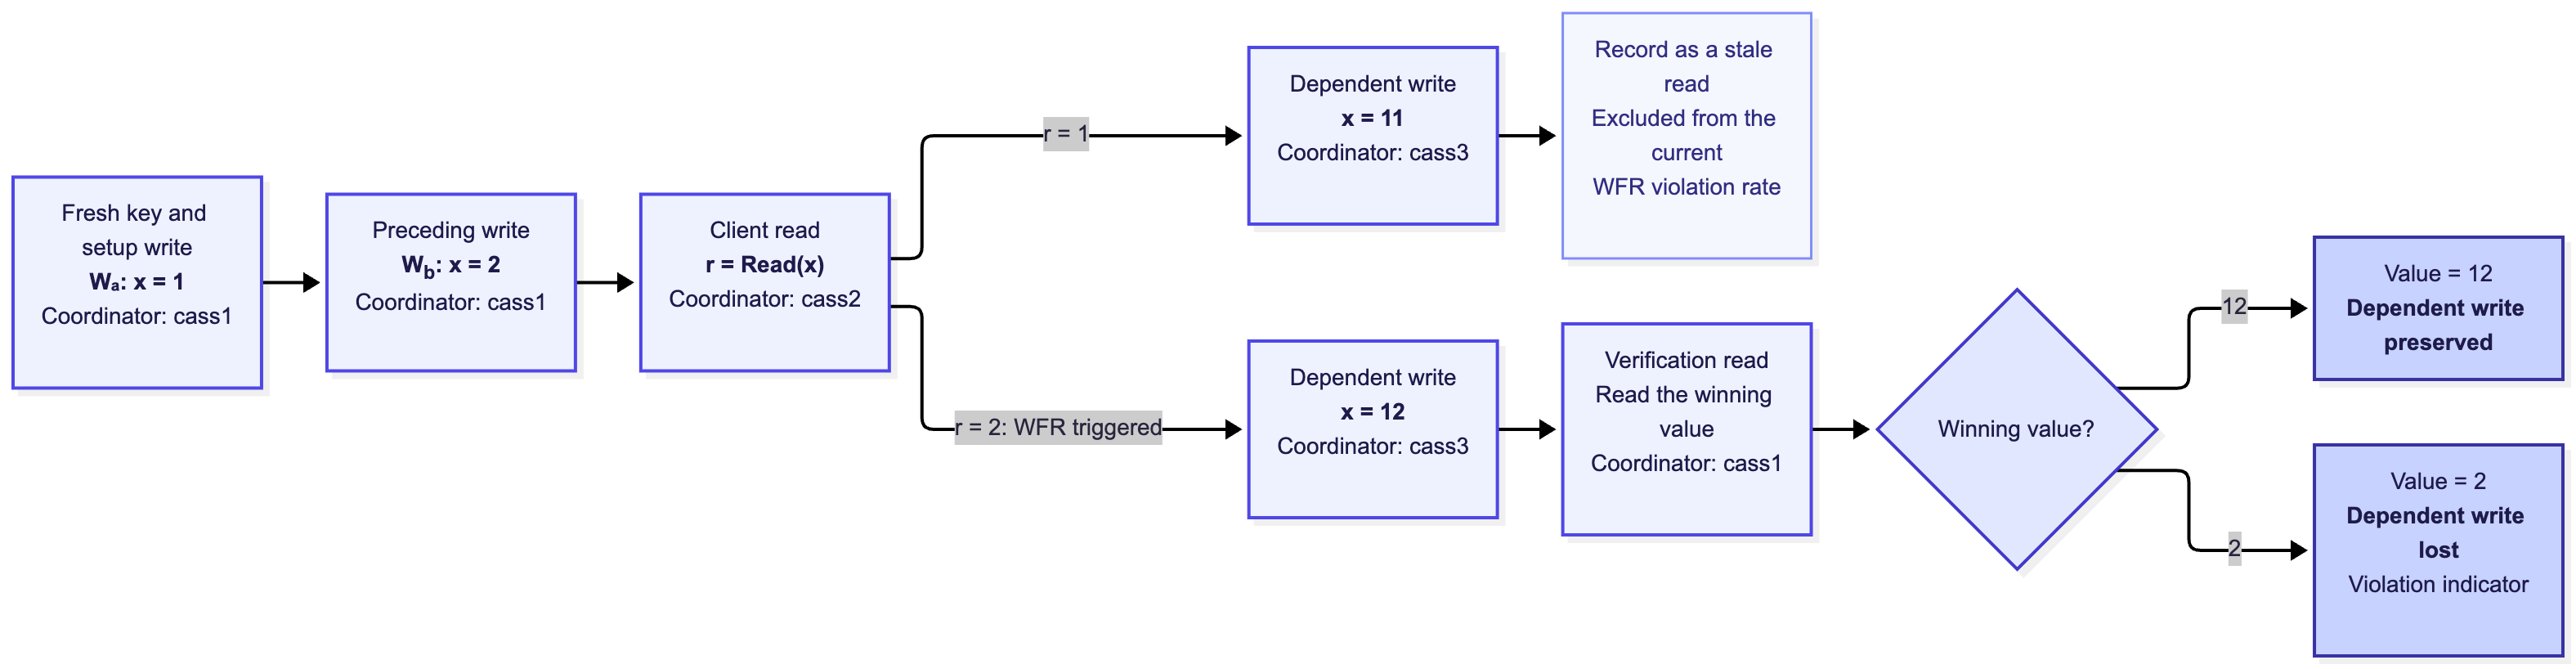
\includegraphics[width=\linewidth]{figures/wfr_flow.png}
\caption{Writes-follow-reads experimental workflow under the normal topology.}
\label{fig:wfr-flow}
\end{figure}

\subsubsection{Principle and Key Implementation}\label{wfr:principle-and-key-implementation}

The analysis distinguishes three outcomes: operation completion, visibility of the preceding write, and preservation of the dependent update.

Operation errors, including unavailable and timeout outcomes, are recorded separately from consistency violations. Among completed trials, the trigger rate measures how often the client reads \(x=2\). The measured WFR violation rate is:

\begin{equation}
\text{Violation rate} =
\frac{\text{triggered trials in which the dependent update is lost}}
{\text{triggered trials}}.
\end{equation}

A configuration with no triggered trials has an undefined violation rate, not a measured rate of 0\%. Such points must therefore appear as gaps in the plots.

For the preceding write and trigger read in natural mode, with RF=3, QUORUM/QUORUM and ALL/ONE satisfy \(R+W>N\), whereas ONE/ONE and ONE/QUORUM do not. Replica overlap helps explain whether the client observes \(W_b\), but it does not determine the ordering of timestamps assigned to competing writes. Even if every replica receives the dependent update, Cassandra's last-write-wins reconciliation can retain \(W_b\) when its timestamp is greater.

\subsubsection{Predicted Outcomes}\label{wfr:predicted-outcomes}

In natural mode, if the dependent write receives a later timestamp than \(W_b\), it should win reconciliation after successful verification. Replication delay may reduce the probability that the preceding read observes \(W_b\), particularly under weak CL combinations, without necessarily causing the dependent update to lose once the test is triggered.

In skew mode, if the future-dated timestamp of \(W_b\) remains greater than that of the dependent write, \(x=2\) should remain the winning value. Increasing the write or read CL should not reverse this timestamp ordering.

{
\begin{table}[H]
\centering
\small
\renewcommand{\arraystretch}{1.15}
\caption{Predicted WFR outcomes conditional on successful operations and a triggered check.}\label{tab:wfr-1}
\begin{tabular}{@{}
  >{\RaggedRight\arraybackslash}p{(\linewidth - 6\tabcolsep) * \real{0.2500}}
  >{\RaggedRight\arraybackslash}p{(\linewidth - 6\tabcolsep) * \real{0.2500}}
  >{\RaggedRight\arraybackslash}p{(\linewidth - 6\tabcolsep) * \real{0.2500}}
  >{\RaggedRight\arraybackslash}p{(\linewidth - 6\tabcolsep) * \real{0.2500}}@{}}
\toprule\noalign{}
\begin{minipage}[b]{\linewidth}\RaggedRight
Timestamp mode
\end{minipage} & \begin{minipage}[b]{\linewidth}\RaggedRight
Condition
\end{minipage} & \begin{minipage}[b]{\linewidth}\RaggedRight
Expected winning value in triggered trials
\end{minipage} & \begin{minipage}[b]{\linewidth}\RaggedRight
Expected measured violation rate
\end{minipage} \\
\midrule\noalign{}
Natural & Dependent write has the later timestamp & 12 & 0\% \\
Skew & \(W_b\) retains the greater timestamp & 2 & 100\% \\
\bottomrule
\end{tabular}
\end{table}
}

These predictions are conditional on successful operations and a triggered check. Failures and partitions are expected to make configurations requiring unreachable replicas unavailable, rather than produce valid consistency observations.

\subsubsection{Results and Analysis}\label{wfr:actual-results-and-analysis}

\paragraph{Delay-scan Results}\label{wfr:delay-scan-results}

\begin{figure}[htbp]
\centering
\begin{subfigure}{\linewidth}
\centering
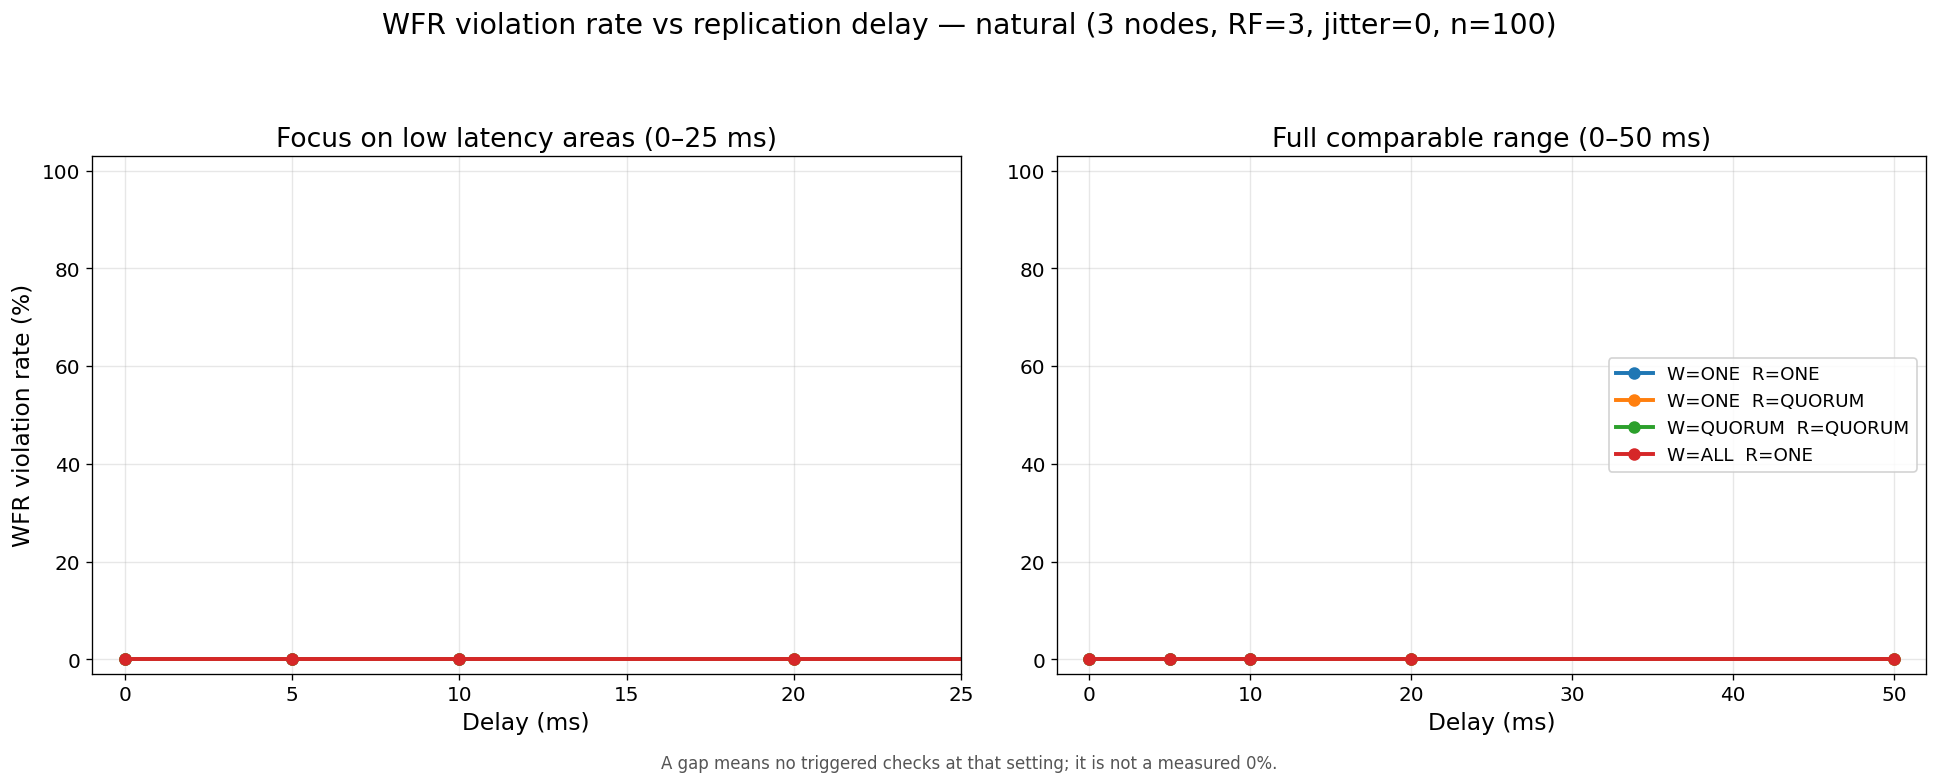
\includegraphics[width=\linewidth]{figures/wfr_natural.png}
\caption{Natural mode}
\end{subfigure}
\par\medskip
\begin{subfigure}{\linewidth}
\centering
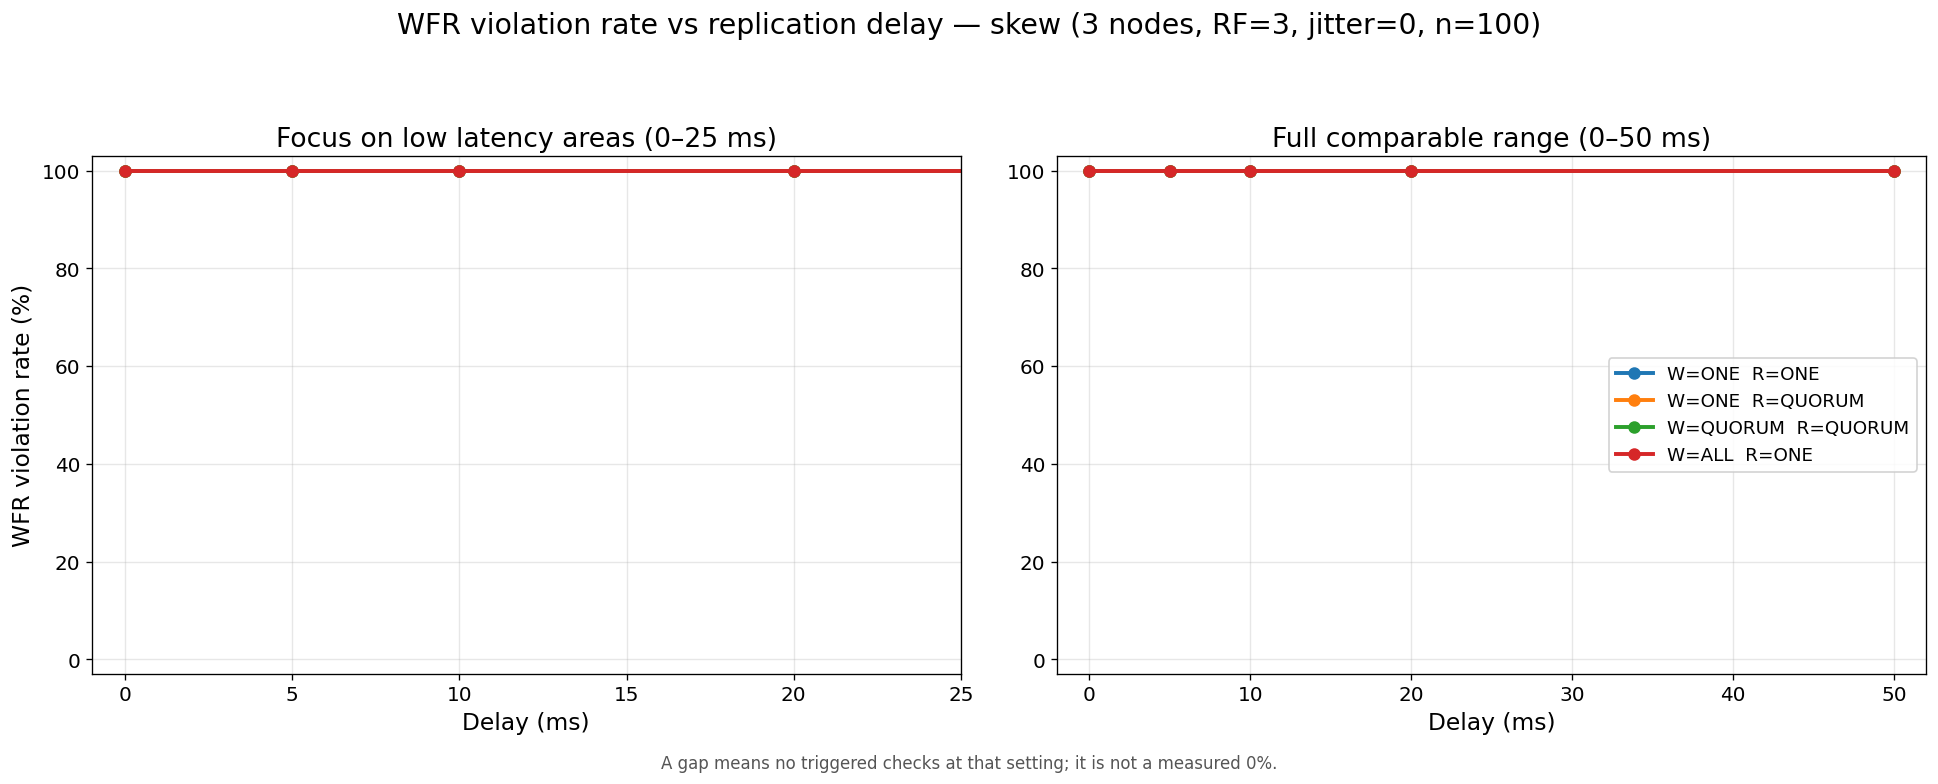
\includegraphics[width=\linewidth]{figures/wfr_skew.png}
\caption{Skew mode}
\end{subfigure}
\par\medskip
\caption{WFR violation rate versus injected replication delay, with RF=3 and jitter=0. Each mode includes a low-delay view and a full displayed range of 0--50 ms. The plots report $n=100$ iterations per configuration; the violation-rate denominator is the number of triggered checks. Gaps indicate settings without triggered checks.}
\label{fig:wfr-delay}
\end{figure}

The delay plots show a clear separation between timestamp modes. In natural mode, all displayed valid observations have a measured violation rate of 0\%. In skew mode, all displayed valid observations have a rate of 100\%. Curves with identical values overlap, so the visible red line should not be interpreted as representing only ALL/ONE. Conversely, an overlapping curve can conceal a gap in another series; a visible line does not establish that every configuration has valid observations at every delay.

Unlike the RYW and MR experiments, the displayed WFR results do not show an increasing violation rate as replication delay grows. This difference follows from the measured event. RYW and MR expose cases in which reads observe missing or older versions during delayed propagation. The WFR indicator is evaluated only after the client has observed \(W_b\), and then checks whether the dependent update survives reconciliation.

In natural mode, the zero-rate observations are consistent with the dependent update receiving a later timestamp and remaining the winner. They do not show that every preceding read was fresh, or that every attempted iteration triggered a WFR check. Replication delay can affect those quantities without changing the conditional violation rate.

The skew-mode results show the opposite outcome. The dependent update loses even under QUORUM/QUORUM and ALL/ONE. Stronger replica acknowledgements therefore do not correct the deliberately inverted timestamp order. This agrees with the MW findings: application order and timestamp order are different, and increasing consistency levels does not make reconciliation follow application order when the supplied timestamps conflict with it.

\FloatBarrier
\paragraph{Results Across Operational Scenarios}\label{wfr:results-across-operational-scenarios}

The original scenario matrix provides complementary evidence about visibility and availability.

{
\begin{table}[H]
\centering
\small
\renewcommand{\arraystretch}{1.15}
\caption{WFR results in the original 64-configuration scenario matrix, excluding the additional delay scan.}\label{tab:wfr-2}
\begin{tabular}{@{}
  >{\RaggedRight\arraybackslash}p{(\linewidth - 10\tabcolsep) * \real{0.1304}}
  >{\raggedleft\arraybackslash}p{(\linewidth - 10\tabcolsep) * \real{0.1739}}
  >{\raggedleft\arraybackslash}p{(\linewidth - 10\tabcolsep) * \real{0.1739}}
  >{\raggedleft\arraybackslash}p{(\linewidth - 10\tabcolsep) * \real{0.1739}}
  >{\raggedleft\arraybackslash}p{(\linewidth - 10\tabcolsep) * \real{0.1739}}
  >{\raggedleft\arraybackslash}p{(\linewidth - 10\tabcolsep) * \real{0.1739}}@{}}
\toprule\noalign{}
\begin{minipage}[b]{\linewidth}\RaggedRight
Mode
\end{minipage} & \begin{minipage}[b]{\linewidth}\raggedleft
Attempted iterations
\end{minipage} & \begin{minipage}[b]{\linewidth}\raggedleft
Completed iterations
\end{minipage} & \begin{minipage}[b]{\linewidth}\raggedleft
Triggered checks
\end{minipage} & \begin{minipage}[b]{\linewidth}\raggedleft
Measured violations
\end{minipage} & \begin{minipage}[b]{\linewidth}\raggedleft
Unavailable or timeout outcomes
\end{minipage} \\
\midrule\noalign{}
Natural & 3,200 & 2,200 & 1,896 & 0 & 1,000 \\
Skew & 3,200 & 2,200 & 2,200 & 2,200 & 1,000 \\
\bottomrule
\end{tabular}
\end{table}
}

These totals refer only to the original 64-configuration matrix, not the additional delay scan.

In natural mode, the 304 completed but untriggered iterations returned the stale value \(r=1\). At zero injected delay, every available configuration achieved a 100\% trigger rate. With 100 ms delay and 50 ms jitter, the normal-topology trigger rate fell to 8\% for ONE/ONE and 79\% for ONE/QUORUM, while QUORUM/QUORUM and ALL/ONE retained 100\%. ONE/ONE also produced low trigger rates under single-node failure and majority partition: 3\% and 6\%, respectively.

These differences are consistent with the replica-overlap argument used in the preceding experiments. ONE/QUORUM can improve visibility relative to ONE/ONE, but \(R+W=N\) does not guarantee overlap. The stronger combinations satisfy \(R+W>N\), consistent with their observed visibility when operations complete. Nevertheless, none of the 1,896 triggered natural-mode checks detected loss of the dependent update.

In skew mode, all 2,200 completed iterations triggered the check and ended with the dependent update losing. The recorded timing checks reported no completed iteration in which the configured skew was too small. The results therefore support the intended timestamp-inversion explanation for this matrix.

Failures and partitions also restricted operation completion. ALL/ONE could not complete after a node failure or within either partition component because all three replicas were not reachable. On the isolated minority, only ONE/ONE completed the WFR sequence. These unavailable outcomes provide availability evidence and must not be interpreted as zero-violation results.

\paragraph{Interpretation and Limitations}\label{wfr:interpretation-and-limitations}

Taken together, the experiments separate visibility, availability, and timestamp ordering. Consistency levels and replication delay affected whether the client observed the preceding write, while network reachability affected whether the sequence could complete. Conditional on a triggered and successfully verified check, the timestamp modes produced opposite outcomes: the dependent update survived in natural mode and lost under the tested timestamp inversion.

The scope of this conclusion is limited by the measurement. The experiment observes the final reconciled value rather than each replica's causal history, and deliberately assigned timestamps do not reproduce all effects of independent machine-clock drift. The displayed scan also covers a finite set of delays and iterations. The results therefore characterize the tested read-dependent-update workload, rather than constitute a complete formal verification of WFR.

\clearpage
\section{Conclusion}\label{conclusion:conclusion}

We tested four client-centric consistency properties in a three-node Cassandra cluster by varying consistency levels, inter-node delay, network availability, and write timestamps. Under weak read and write settings, delayed propagation exposed read-your-writes and monotonic-reads violations when the client accessed different coordinators. QUORUM/QUORUM and ALL/ONE produced no observed violations in the corresponding successful read experiments. ONE/QUORUM gave mixed results: RYW violations occurred in some runs, while no MR violations were observed under the tested paths and schedules. The latter result does not establish a general MR guarantee.

The monotonic-writes experiment showed that natural timestamp ordering preserved the intended final overwrite in all successful trials. When we deliberately assigned the earlier write a greater timestamp, that write won every successful verification read, regardless of the write consistency level. This measures the final reconciled value, rather than the order in which each replica applied the writes. In the writes-follow-reads experiment, no loss of the dependent write was observed in 1,896 natural-mode trials that read the target version. With inverted client timestamps, the dependent write lost in all 2,200 triggered trials, including those using stronger consistency levels.

Failures and partitions also changed which operations could complete. A majority partition could still serve quorum requests, whereas the isolated node could complete only operations that required a single replica. Taken together, these results show that consistency levels affect visibility and availability, while timestamp ordering determines the winner of competing writes in our MW and WFR tests. The findings describe the observed workloads and success conditions; they do not constitute a formal verification of the four consistency properties.

\clearpage
\appendix
\section{AI Tool Declaration}\label{app:ai-declaration}

We acknowledge the use of Claude (Anthropic) and ChatGPT/Codex (OpenAI) in preparing this project. These tools were used for assistance with implementation, visualisation, and report preparation, as described below.

\subsection*{Claude}
Claude assisted with developing the Cassandra experiment infrastructure and framework, including the three-node Docker configuration, node-pinned client sessions, parameterised consistency tests, timestamp-inversion tests, and internode latency-injection scripts. The repository's initial framework commit explicitly credits ``Claude Opus 5'' in its co-author attribution. This attribution can be inspected in \href{https://github.com/LuweiChenbot/Cassandra-Lab/commit/261a1f4a33a35dfb7b4157cd4addb2c38258370b}{commit \texttt{261a1f4}} of the project repository.

\subsection*{ChatGPT/Codex}
ChatGPT/Codex was used as an supporting tool for proofreading grammatical errors in the report, improving formatting and presentation, reviewing the project code for consistency with the assignment requirements, and refining the clarity, organisation, and expression of the written report.

\subsection*{Responsibility for the submission}
AI assistance does not replace experimental evidence, database documentation, or the authors' responsibility for scientific judgement. The reported measurements must be supported by the experiment outputs and not by AI-generated assertions. We are responsible for checking AI-assisted code, interpretations, references, and written material, and for the content, accuracy, originality, and quality of the submitted work.

\end{document}
